\documentclass[11pt,letterpaper]{scrartcl}
\usepackage[secthm,mdthm,simplethm]{beel}
\usepackage{graphicx}
\usepackage{tcolorbox}
\usepackage[margin=1in,top=0.8in,bottom=0.8in]{geometry}
%%%%%%Packages%%%%%%%%%%%%%
\usepackage{amsmath}
\usepackage{amsfonts}
\usepackage{amsthm}
\usepackage{amssymb}
\usepackage{array}
\usepackage{comment}
\usepackage{enumitem}
\usepackage{graphicx}
\usepackage{hyperref}
\usepackage[utf8]{inputenc}
\usepackage{mathtools}
\usepackage{multicol}
\usepackage{tabto}
\usepackage{tikz}
\usepackage{pgfplots}
\usepackage{setspace}
\usepackage[all]{xy}
\usepackage{thmtools}
\usepackage{MnSymbol,wasysym}
%%%%Theorem Enviorment Setup%%%%%%%
\begin{comment}
\theoremstyle{definition}
\newtheorem{theorem}{Theorem}[section]
\newtheorem{corollary}{Corollary}[theorem]
\newtheorem{lemma}[theorem]{Lemma}
\newtheorem{claim}[theorem]{Claim}
\newtheorem{definition}{Definition}[section]
\newtheorem{example}{Example}[section]
\newtheorem{remark}{Remark}[section]
\newtheorem{proposition}[theorem]{Proposition}
\end{comment}
\pgfplotsset{compat = 1.15}
%%%%%%%%%HyperLink Setup%%%%%%%%%%%
\hypersetup{
    colorlinks=true,
    urlcolor=blue,
}
%%%%%%%%%%%%%%%Commands%%%%%%%%%%%%%%%%
\newcommand{\pml}{\left( \begin{array}{rrrrr}}
\newcommand{\pmr}{\end{array} \right) }
\newcommand{\bml}{\left[\begin{array}{rrrrr}}
\newcommand{\bmr}{\end{array} \right]}
\newcommand{\aml}{\left[ \begin{array}{rrr|r}}
\newcommand{\amr}{\end{array} \right]}
\newcommand{\vml}{\left\vert \begin{array}{rrrrrrrrrr}}
\newcommand{\vmr}{\end{array} \right\vert}
\renewcommand{\tab}{\hspace{1cm}}
\renewcommand{\b}{\mathbb}
\renewcommand{\c}{\mathcal}
\newcommand{\lb}{\left\{}
\newcommand{\rb}{\right\}}
\newcommand{\la}{\langle}
\newcommand{\ra}{\rangle}
\renewcommand{\bar}{\overline}
\newcommand{\ngroup}{\trianglelefteq}
\newcommand{\ver}{ \ | \ }
\renewcommand{\t}{\text}
\newcommand{\z}{\mathbb Z}
\renewcommand{\r}{\mathbb R}
\newcommand{\q}{\mathbb Q}
\newcommand{\ex}{\textbf{Example. }}
\renewcommand{\mod}[1]{\t{ (mod } {#1})}
\newcommand{\zz}[1]{\b Z/ {#1} \b Z}
\newcommand{\cg}[1]{\la {#1} \ra}
\newcommand{\li}[2]{{#1}_1,{#1}_2, \ldots, {#1}_{#2} }
\renewcommand{\v}{\vec}
\renewcommand{\t}{\tilde}
\newcommand{\spa}{\text{span}}
%%%%%%%%%%%% main doc%%%%%%%%%%%%
\begin{document}
\centerline{\huge \textbf{Math 110, Spring 2019}} 
\vskip 0.6cm
\thispagestyle{empty}
\tableofcontents
\newpage
%!TEX root = ./main.tex
\section{Vector Space}
\subsection{Vector Space over a field and subspace}
Recall that $(\b F, + , \cdot)$ or $\la \b F, + , \cdot \ra$, where $\b F$ is a set, and $+ , \cdot $ are binary operations. \\
We know that $(\b F, +)$ and $(\b F \ \backslash \lb 0 \rb, \cdot)$ and $+, \cdot $ satisfy distributivity.
\begin{definition}
$V$ is a vector space over a field $\b F$ is $V$ is equipped with vector addition $+ : V \times V \to V$ and scalar multiplication $\cdot : \b F \times V \to V$.
\end{definition}
\subsubsection*{Lists (and vector spaces of lists)}
\begin{example} 
$\b R^n, \b C^n$, or generally $\b F^n$. 
\[ \b R^{n} = \lb (x_1,x_2, \cdots x_n) : x_i \in \b R \ \forall \ j = 1,2 \cdots n \rb \]
\[ \b F^{n} = \lb (x_1,x_2, \cdots x_n) : x_i \in \b F \ \forall \ j = 1,2 \cdots n \rb \]
\end{example}
\noindent We claim that $\b F^n$ is a vector space over $\b F$ provided $\b F$ is a field. We can define addition and scalar multiplication as 
\[ (\li xn) + (\li yn) := (x_1 + y_1, x_2 + y_2, \cdots , x_n + y_n)\]
\[ \alpha \cdot (\li xn) =  ( \alpha \cdot x_1, \alpha \cdot x_2, \cdots, \alpha \cdot x_n)\ \ \ \alpha \cdot x_i \in \b F\]
\textbf{What rules / axioms should we impose?}
\begin{itemize}
    \item Commutativity \\
    $\vec v + \vec w = \vec w + \vec v \ \forall \ \vec v,\vec w \in V$. 
    \item Associativity \\
    $(\vec v + \vec w) + \vec u = \vec v + (\vec w + \vec u) \ \forall \ \vec v, \vec w, \vec u \in V$. 
    \item Additive Identity \\
    $\exists \ \vec 0 \in V : \vec v + \vec 0 = \vec v + \vec 0 = \vec v$ 
    \item Additive Inverse
    $\forall \vec v \in V \ \exists \ \vec w \in V : \vec v + \vec w = \vec 0$.
    \item (Mixed) Scalar Multiplication Rules \\
    $1 \cdot \vec v \in \vec v \tab \forall v \in V$
    \item Distributivity:  \\
    $(\alpha + \beta ) \cdot \vec v = \alpha \cdot \vec v + \beta \cdot \vec v \tab \forall \ a,b, \in \b F \tab \forall \ \vec v \in V$ \\
    $\alpha \cdot (\vec v + \vec w) = \alpha \cdot \vec v + \alpha \cdot \vec w \tab \forall \ a \in \b F \tab \forall \ \vec v ,\vec w \in V$
\end{itemize}
Now we can check that these rules hold in $\b F^2$:
\begin{align*}
    (0,0,\cdots,0) + (\li xn) &= (\li xn) \\
    (\li xn) + (\li{-x}n) &= (0,0,\cdots,0) 
\end{align*} \\
\textbf{Basic Observation}  
$\vec 0$ is unique 
\begin{proof}
    Suppose $\vec 0_1$ and $\vec 0_2$ are both identity element with respect to $+$:
    \[ \vec 0_1 = \vec 0_1 + \vec 0_2 + \vec 0_2\]
    A contradiction.
\end{proof}
Additive inverse ate unique, i.e., if $\vec v + \vec w = \vec 0$ and $\vec v + \vec w = 0$, then $\vec u = \vec w$. 
\begin{proof}
    Suppose $\vec v + \vec w = \vec 0$ and $\vec v + \vec w = \vec 0$, then
    \[\vec w = \vec w + \vec 0 = \vec w + (\vec v + \vec u) = (\vec w + \vec v) + \vec u = \vec 0 + \vec u = \vec u\]
    A contradiction.
\end{proof}
\noindent \textbf{Additive Inverse} 
\begin{align*}
    (-1) \cdot \vec v + \vec v &= (-1) \cdot \vec v + 1 \cdot \vec v \\
    &= ((-1) + 1) \cdot \vec v \\
    &= 0 \cdot \vec v \\
    0 \cdot \vec v + 0 \cdot \vec v &= (0 + 0) \cdot \vec v \\ &= 0 \vec v \implies \boxed{ 0 \cdot \vec v = \vec 0}
\end{align*} 
Additive inverse $\implies$ $0 \cdot \vec v = \vec 0$ on both sides. 
\subsection{Subspaces}
\begin{definition}
    $V$ is a vector space over a field $\b F$, Let $W \subseteq V$. \\
    $W$ is called a subspace of $V$ if $W$ equipped with the same operations $+, \cdot$ inherited from $V$ is still a vector space.
\end{definition}
\textbf{Is it enough for $W$ to be just a subset of $V$?} \\
Suppose $V = \b R^3$ is a vector space over $\b R$. Let $W := \lb (1,1,1) \rb$, the additive inverse doesn't exist. Note that $W$ is not closed in addition and scalar multiplication. \\
\[W := \lb (x,0,0) \ : \ x_1 \in \b R \rb\]
\textbf{Why is $\vec 0$ in every subspace?} \\
We know that a vector space is a \textit{non empty} set, and $W$ is closed under multiplication, so since $0 \in \b F$, therefore $0 \cdot \vec v = \vec 0 \in W$. 
\begin{remark}
If $\vec v + \vec w = \vec v$, for some $\vec v \in V$, then $\vec w = \vec 0$.
\end{remark}
\begin{proof}
    Suppose $\vec v + \vec w = \vec v$, then $- \vec v + \vec v  +\vec w = - \vec v + \vec v \implies \vec 0 + \vec w = \vec 0 \implies \vec w = \vec 0$
\end{proof}
We recall that $\b F^n$ is defined as 
\[\b F^n = \lb (\li xn)\ : \ x_i \in \b F \rb \]
We can define $\b F^S$ for $S$ being a set as $\b F^{S} = \lb f :  \underbrace{S}_{\text{no structure needed}} \to \underbrace{\b F}_{\text{field}} \rb $ \\
We can define addition and multiplication as
\[ (f + g)(s) := f(s) + g(s) \ \forall s \in S \]
\[ (\lambda \cdot f)(s) := \lambda \cdot f(s) \in \b F\]
Suppose $S = \lb 1,2,3 \rb$, what is $\b F^S$ or $\b R^S$?
We can thought of $\b R^S$ as $\b R^3$..... why?
\begin{remark}
    We can conclude $\b F^S \cong \b F^{|S|}$, where $|S|$ is the cardinality of $S$. If $S$ is finite.
\end{remark}
What is $\b R^{\b N}$? $\leftarrow$ the set of all of all real sequences.
\begin{remark}
    In the book we uses $\b R^\infty$, we can conclude that \[ \b R^\infty \cong \b R^{\b N} \]
\end{remark}
We say that $W$ is a subspace of $\b R^\infty$ with $+, \cdot$
\[ W := \lb s \ : \ \lim_{n \to \infty} s(n) = 0 \rb \]
\begin{proof}
    We can see that if $\displaystyle \lim_{n \to \infty} s(n) = 0$ and $\displaystyle \lim_{n \to \infty} t(n) = 0$, then $\displaystyle \lim_{n \to \infty} (s + t)(n) = 0 $. \\
    If $\lambda \in \b R$, then $\displaystyle \lim_{n \to \infty} s(n) = 0 \implies \lim_{n \to \infty} (\lambda \cdot s)(n) = 0$. \\ The zero sequence is in $W$ so $\vec 0 \in V$. Therefore $W$ is a subspace of $V$.
\end{proof}
\begin{theorem}
    $W$ is a subspace of $V$ iff $W$ is closed under addition, multiplication by scalar multiplication by scalars, and $\vec 0 \in V$.
\end{theorem}
Since the operation in inherent from vector space $V$, we do not need to verify the other property since they all for all $V$ and $W$ is a subspace of $V$. \\
\textbf{How do we form new subspaces from existing ones?}

\begin{theorem}
    Suppose $W_1,W_2$ are subspaces of $V$, then $W_1 \cap W_2$ is a subspace of $V$.
\end{theorem}
\begin{proof}
    We know that $W_1,W_2$ are subspaces of $V$, therefore $\vec 0 \in W_1$ and $\vec 0 \in W_2$, then $0 \in W_1 \cap W_2$. \\
    Suppose $\vec v,\vec u \in W_1 \cap W_2$, we know that $\vec v,\vec u \in W_1$ and $\vec v, \vec u \in W_2$. Since $W_1,W_2$ is a subspace, therefore $\vec u + \vec v \in W_1 \land \vec u + \vec v \in W_2 \implies \vec u + \vec v \in W_1 \cap W_2$, therefore $W_1 \cap W_2$ is closed under vector addition. \\ 
    Suppose $\alpha \in \b F$ and $\vec v \in W_1 \cap W_2$. We know that $\alpha \cdot \vec v \in W_1$ and $\alpha \cdot \vec v \in W_2$ since they are both subspaces of $V$. Therefore we conclude $\alpha \cdot \vec v \in W_1 \cap W_2$, therefore $W_1 \cap W_2$ is closed under multiplication. \\
    Therefore $W_1 \cap W_2$ is a subspace of $V$.
\end{proof}
\begin{proposition}
    The union of two subspace of $V$ are generally not a subspace of $V$
\end{proposition}
\begin{proof}
    We can see that $\text{span} \lb \vec e_1 \rb$ and $\text{span} \lb \vec e_2 \rb$ is not a subspace if $\b R^2$ as $(1,1) \not\in W_1 \cup W_2$ 
\end{proof}
\begin{theorem}
    Union of two subspaces of $V$ is a subspace of $V$ if and only if one of the subspaces is contained in the other.
\end{theorem}
\begin{proof}
    The proof is left as an exercise.
\end{proof}
\begin{theorem}
    $W_1 + W_2$ is a subspace of $V$.
\end{theorem}
\begin{proof}
    (identity) $\vec 0 \in W_1 \land \vec 0 \in W_2 \implies \vec 0 + \vec 0 = \vec 0 \in W_1 + W_2$. \\
    (closure under addition) Suppose $\vec w_1 + \vec w_2 \in W_1 + W_2$ and $\tilde{\vec w}_1 + \tilde{\vec w}_2 \in W_1 + W_2$. We compute $(\vec w_1 + \vec w_2) + (\tilde{\vec w}_1 + \tilde {\vec w}_2) = \underbrace{(\vec w_1 + \tilde{\vec w}_1)}_{\in W_1} + \underbrace{(\vec w_2 + \tilde{\vec w}_2)}_{\in W_2} \implies (\vec w_1 + \vec w_2) + (\tilde{\vec w}_1 + \tilde{\vec w}_2) \in W_1 + W_2$. \\

    (closure under scalar multiplication) Suppose $\vec w_1 + \vec w_2 \in W_1 + W_2$, and $\lambda \in \b F$, we compute $\lambda \cdot (\vec w_1 + \vec w_2)  = \underbrace{(\lambda \cdot \vec w_1)}_{\in W_1} + \underbrace{(\lambda \cdot \vec w_2)}_{\in W_2} \implies \lambda \cdot (\vec w_1 + \vec w_2) W_1 + W_2$
\end{proof}
\begin{remark}
    $W_1 + W_2 + \cdots + W_n$ if the smallest subspace containing $\li Wn$. \\
    If $\tilde {\vec v}$ is a subspace of $V \supseteq W_j \ \forall j$, since $\tilde {\vec v}$ is closed under $+$, $\vec w_1 + \vec w_2 + \cdots + \vec w_n \in W_n$
\end{remark}
\begin{example}
Suppose $V = \b R^3$. Let \[W_1 = \spa \{\vec e_1, \vec e_2\}, W_2 = \spa \{(0,1,1)\}, W_3 = \spa \lb (x,y,z) : x + y + z = 0 \rb\] 
What is $W_1 + W_2 + W_3$?
\end{example}
Note that $(0,0,1) = \underbrace{\left(0,\frac12,\frac12\right)}_{\in W_2} +  \underbrace{\left(0,-\frac12,\frac12\right)}_{\in W_3}$. We also know that $(1,0,0) \in W_1$ and $(0,1,0) \in W_2$, therefore $W_1 + W_2 + W_3 = \b R^3$ \\
\section*{Discussion}
\begin{definition}
    A vector space, is often denoted as $(\underbrace{\b F}_{\text{scalars}}, \underbrace{V}_{\text{vectors}}, \cdot : \underbrace{\b F \to B}_{scaling})$
\end{definition}
\begin{example}
    $(\b R,\b R^n, \cdot : \b R \times \b R^n \to \b R^n)$ is a vector space.
\end{example}
\begin{example}
    $(\b R, \b R, \cdot : \b R \times \b R \to \b R)$ is also a vector space.
\end{example}
\subsubsection*{Notion of a field}
Suppose $F  = \lb 0,1,2,3 \rb$. Can $F$ be a field?
\begin{definition}
    A subset $W$ of the vector space $V$ is a subspace of $V$ if it satisfy the following:
    \begin{enumerate} [label  = \arabic*)]
        \item $\vec 0 \in W$ 
        \item $+ : W \times W \to W \subseteq V$ (closure under addition)
        \item $\cdot : \b F \times W \to W \subseteq V$ (closure under scalar multiplication)
    \end{enumerate}
\end{definition}
\begin{example}
    Can we find a subset $W$ of $V$ such that $W$ satisfy property 1), 2) but not 3)? \\
    Suppose $W  =\lb (x,0) : x \in \b Z\ \rb$ the proof is trivial and is left as an exercise.
\end{example}
\begin{example}
    The set of functions $\lb f : (0 ,\infty) \to \b R \rb = \b R^{(0,\infty)}$ is a vector space. We claim that $W$ is a subspace of $V$.
    \[ W = \lb f : (0,\infty) \to \b R : f'(1) = 0 \rb\]
\end{example}
\begin{proof}
    We begin by verifying the three properties
    \begin{enumerate} [label  = \arabic*)]
        \item The zero function is in $W$
        \item Suppose $f,g \in W$, then $(f + g)'(1) = f'(1) + g'(1) = 0 + 0 = 0 \implies f(x) + g(x) \in V$
        \item Suppose $f \in W$ and $\lambda \in \b F$, then $\lambda \cdot f'(1) = \lambda \cdot 0 = 0 \implies \lambda \cdot f(x) \in V$
    \end{enumerate}
    Therefore $W$ is a subspace of $V$. 
\end{proof}
\subsection{Direct Sum}
\begin{definition}
    Let $(\b F, V, \cdot : \b F \times V \to V)$ be a vector space. Given that $\li Un \subseteq V$ are subspaces of $V$, we can define the sum of the subspaces as 
    \[ U_1 + U_2 + \cdots + U_n = \lb \vec u_1 + \vec u_2 + \cdots + \vec u_n : \vec u_i \in U_i \rb \]
\end{definition}
\begin{proof}
    \begin{enumerate} [label  = \arabic*)]
        \item We can see that $\vec 0 \in U_i \ \forall i$, and $\vec 0 + \vec 0 + \cdots + \vec 0 = \vec 0$
        \item Suppose $\vec x = \sum_{i = 1}^n \vec x_i \in U_i$ and $\vec  y = \sum_{j = 1}^n \vec y_j \in U_j$, we can see that $\vec x + \vec y = \sum_{k = 0}^n \vec x_k + \vec y_k \in U_k$, therefore it's closed under addition.
        \item Suppose $\lambda \in \b F$ and $\vec x = \sum_{i = 1}^n \vec x_i \in U_i$, we compute $\lambda \cdot \vec x = \lambda \cdot \sum_{i = 1}^n \vec x_i \in U_i$, therefore it's closed under scalar multiplication.
    \end{enumerate}
\end{proof}
\begin{definition}
    We say that $U_1 + U_2 + \cdots + U_n$ is a direct sum, denoted as $U_1 \oplus U_2 \oplus \cdots \oplus U_n$ if for every $\vec v \in U_1 + U_2 + \cdots + U_n$, $\vec v = \vec u_1 + \vec u_2 + \cdots + \vec u_n$ has a unique representation. 
\end{definition} 
\begin{remark}
    How best to check $U_1 + U_2 + \cdots + U_n$ is a direct sum? \\
    Check that $U_i \cap U_j = \lb \vec 0 \rb$. We will go over in depth later.
\end{remark}
What about $W_1 + W_2 + \cdots W_n$ being a direct sum?
\begin{theorem}
    The sum of subspaces $\li Wn$: 
    \[W_1 + W_2 + \cdots + W_n\]
    is a direct sum iff $\vec 0$ can be written in only \textbf{one way} as a sum 
    \[ \vec w_1 + \vec w_2 + \cdots + \vec w_n = 0\]
    namely $\vec 0 + \vec 0 + \cdots + \vec 0 = \vec 0$.
\end{theorem}
\begin{remark}
    If $W_1 \cap W_2 \neq \lb \vec 0 \rb, W_1 \cap W_3 \neq \lb \vec 0 \rb, W_2 \cap W_3 \neq \lb \vec 0 \rb$, it is not possible for $W_1,W_2,W_3$ to be a direct sum, However, the opposite of the proposition is not sufficient for being a direct sum as demonstrated in Remark 1.25.
\end{remark}
\begin{remark}
    $W_1 \cap W_2 = \lb \vec 0 \rb$, $W_1 \cap W_2 = \lb \vec 0 \rb$, $W_2 \cap W_3 = \lb \vec 0 \rb$ and $W_1 + W_2 + W_3$ being not a direct sum is possible. For example, consider $\b R_2$, for line $x = y, y = 0$ and $x = 0$, we can see that they only have the trivial intersection but they are not a direct sum. (credit: Catherine)
\end{remark}
\newpage  \vfill
%!TEX root = ./main.tex
\section{Finite Dimensional Vector Spaces}
\subsection{Linear Dependence and Independence} 
\begin{definition}
    We will works with lists of vectors $\li vk$, then the span of $\li vk$ can be defined as
    \begin{align*}
         \spa (\li{\vec v}k) &:= \lb \alpha_1\vec v_1 + \alpha_2 \vec v_2 + \cdots  + \alpha_k \vec v_k \rb  \forall \alpha_i \in \b F 
    \end{align*}
    If the the list happens to cover the entire vector space $V$, we call the list a spanning list of $V$.
\end{definition}
\begin{definition}
    $V$ is finite dimensional if $V$ is a span of finitely many vectors.
\end{definition}
\begin{remark}
    $V$ is not finite dimensional is logically equivalent to $V$ is infinite dimensional.
\end{remark}
\begin{example}
    Consider the vector spaces: $\c P(x) : = \lb \alpha_0 + \alpha_1 x + \cdots + a_kx^k : a_j \in \b F \text{ for some } k \rb$. We can see that $\c P(x) \subseteq \b F^{\b F}$, and $\c P(x)$ is infinite dimensional.
\end{example}
\begin{definition}
    We can define the degree of a polynomial, denoted as $\deg(f(x))$, is the highest power of $x$ where hose coefficient ($\alpha_k$) is nonzero. The zero function $f(x) = 0$ has $-\infty$ degree. 
\end{definition} 
\begin{example}
    $\c P(x)$ is infinite dimensional.
\end{example}
\begin{proof}
    Suppose $\c P(x) = \text{span}(\li fk)$, where $f_j$ is polynomials, for all $j$. 
    Let \[D := \text{max}\lb\deg(f_1), \deg(f_2), \cdots, \deg(f_k)\rb\] Suppose $f(x) =  x^{D + 1} \in \c P(x)$ however, $x \not\in \text{span}(\li fk)$. Since $f(x)$ is not a linear combination of $\li fk$. A contradiction, therefore $\c P(x)$ is a infinite dimensional vector space.
\end{proof}
\begin{definition}
    $V$ has dimension $k$ over $\b F$ if you can find vectors $\li vk$ such that
    \[\forall \vec v \in V : \vec v = \sum f_i\vec v_i \text{ uniquely}\]
\end{definition}
\begin{definition}
    $\c P_d(x) : =$ all polynomials in $g(x)$ of degree $\leq d$. \\ Note that $\{ 1, x, x^2, \cdots, x^d\}$ is a spanning list for $\c P_d(x)$
\end{definition}
\begin{definition}
    A list $\li {\vec v}k \in V$ is called \textbf{linearly independent} if the equation
    \[ \alpha_1 \vec v_1 + \alpha_2 \vec v_2 + \cdots + \alpha_k \vec v_k = 0 \implies \li \alpha k = 0\]
\end{definition}
\begin{definition}
    A list $\li {\vec v}k \in V$ is called \textbf{linearly dependent} if it is not independent.
\end{definition}
\subsection*{Digression on Logic}
Logic: $A \implies B$ is equivalent to $\neg A \lor B$. Then we know that \[\neg (A \implies B) \iff (\neg(\neg A \lor B)) \iff A \land \neg B\]
\begin{definition}[The better definition]
    A list $\li {\vec v}k \in V$ is called \textbf{linearly dependent} if for equation
    \[ \alpha_1 \vec v_1 + \alpha_2 \vec v_2 + \cdots + \alpha_k \vec v_k = 0\] has a nontrivial solution such that $\li {\vec v}k \neq 0$
\end{definition}
\begin{example}
    Is $\lb \rb$ linearly independent? \\
    By definition, it is linearly independent, because it is not linearly dependent. A set $S$ is linearly dependent if there exists a finite set of vectors $\li {\vec v}n$ and corresponding scalars $\li \alpha n$ such that there exists at least one $\alpha_i \neq 0$ so that \[ \sum_{i= 0}^n \alpha_i \vec v_i = 0\] since $\alpha_i$ doesn't exist, we know that $\lb \rb$ is linearly independent.
\end{example}
\begin{example}
    Is $\lb (1,0,0),(0,1,0),(0,0,1)\rb$ linearly independent on $\b R^3$?
    \begin{align*}
        \alpha_1(1,0,0) + \alpha_2(0,1,0) + \alpha_3(0,0,1) &= (0,0,0) \\
        \implies (\alpha_1, \alpha_2, \alpha_3) &= (0,0,0) \\
        \implies \alpha_1 = \alpha_2 = \alpha_3 &= 0
    \end{align*}    
\end{example}
\begin{remark}
    We can remove vectors from a linearly independent list can still remain independent, however, we cannot guarantee the result if we are still adding vectors; In mathematical terms, any sublist of the list is linearly independent, since $\lb \rb$ is a sublist of any list, therefore its linearly independent.
\end{remark}
\begin{lemma}[Linear Dependence Lemma]
    Suppose $\li {\vec v} h$ is linearly independent. Then there exists $j$ between $1$ and $k$ such that 
    \begin{itemize}
        \item $v_j \in \spa \lb \vec v_1, \vec v_2, \vec v_{j-1} \rb$
        \item $\spa \lb \li {\vec v} h \rb = \spa \lb \li {\vec v}{j-1}, \vec v_{j+1} , \cdots, \vec v_k \rb$
    \end{itemize}
\end{lemma}
\begin{proof}
    If $\li{\vec v}k$ is a linearly dependent list, there are coefficients $\li \alpha k$ not all $0$, such that 
    \[ \alpha_1 \vec v_1 + \alpha \vec v_2 + \cdots \alpha_k \vec v_k = 0\]
    Take $j$ such that $\alpha_j$ is the largest index with $\alpha_j \neq 0$. Then $\alpha_{j + 1}=  \alpha_{j + 2} = \cdots = \alpha_k = 0$ and \[ \vec v_j = \frac{-1}{\alpha_j} (\alpha_1 \vec v_1 + \alpha \vec v_2 + \cdots + \alpha_{j - 1} \vec v_{j-1})\] hence $\vec v_j \in \spa \lb \li{\vec v}{j-1} \rb$.
\end{proof}
\begin{lemma}[Very Important, a.k.a. Magic Lemma]
    The length of the independent list $\leq$ length of any spanning list. 
\end{lemma}
\begin{proof}
    Say $\li {\vec u}n$ is linearly independent say $\li {\vec v} m$ is spanning. Then we want to establish that $ m \leq n$. 
    \begin{enumerate}[label = {Step \arabic*.}]
        \item Take the list $\vec u_1, \li {\vec v} m$ It is linearly independent since $\vec u_1 \in \spa \lb \li {\vec v}m \rb$. By the linear dependence lemma, there is a $j$ such that $\vec v_j$ can be removed (noted that $\vec u_1$ cannot be subject to removal since $\vec u_1$ comes from a linearly independent list). Consider the new list $\lb \vec u_1, \li {\vec v}{j-1} , \cdots, \vec v_m\rb$
        \item We can continue this process by bringing $\vec u_2, \vec u_3, \cdots \vec u_n$, we know that $\vec u_i$ since they are linearly independent.
    \end{enumerate}
    Note that this process preserves linear span of the whole list.  \\
    We know that this list contains all the $\vec u_i$ (plus possibly some remaining $\vec v_j$) and the length of the list is always $n$. So $\boxed{m \leq n}$.
\end{proof}
\subsection{Bases and Dimension}
\begin{definition}
    A basis a linearly independent spanning list.
\end{definition}
\begin{theorem}
    Any two basis in a finite dimensional space have the same number of vectors.
\end{theorem}
\begin{remark}
    The span of $\lb \rb$ is the zero vector.
\end{remark}
\begin{theorem}
    Suppose $V$ is a finite dimensional vector space. Let $W$ be a subspace of $V$, then $W$ is finite dimensional.
\end{theorem}
\begin{proof}
    $V$ is finite dimensional means that $V$ is spanned by some $k$ vectors. Consider $W$. If $W = \lb \vec 0 \rb$, then $w$ is spanned by the empty list $\vec 0$. If $W \neq \vec 0$, there exists $\vec w_1 \in W$ such that $W = \spa\lb \vec u_1 \rb$, done. Otherwise take $\vec w_2 \in W \ \backslash \  \spa \lb \vec w_1 \rb$. Repeat this algorithm until it terminates. Now we want to show that this algorithm will terminate at $\vec w_k$, we know that $\li {\vec w}j$ is linearly independent by construction and the linearly dependence lemma. By remark 2.16, we know that the length of any such list will not exceed length $k$, therefore we know the algorithm will terminate in finite steps. This implies that $W$ is finitely spanned, or $W$ is finite dimension.
\end{proof}
\subsubsection{Dimension}
\begin{definition}
    Dimension of a vector space $V$ is the cardinality of any basis in a finite dimensional space.
\end{definition}
\begin{proposition}[Criterion for a Basis]
    $\li {\vec v}k$ is a basis for $V$ if and only if any $v \in V$ can be uniquely written as a lineat combination
    \[ \lambda_1 \vec v_1 + \lambda_2 \vec v_2 + \cdots + \lambda \vec v_n \]
\end{proposition}
\begin{proof}
    We know that ``can be written  as linear combination" is logically equivalent a $\li {\vec x} k$ is a spanning list for $V$. ``uniqueness" is logically equivalent as linear independence. Suppose
    \[ \vec v = \alpha_1 \vec v_1 + \alpha_2 \vec v_2 + \cdots + \alpha_k \vec v_k = \beta_1 \vec v_1 + \beta_2 \vec v_2 + \cdots + \beta_k \vec v_k\]
    Not all $\alpha_j = \beta_j$. Then $(\alpha_1 -\beta_1) \vec v_1 + (\alpha_2 - \beta_2) \vec v_2 + \cdots (\alpha_k - \beta_k) \vec v_k = \vec 0$ is a nontrivial linear combination of $\li {\vec v} k$ and vice versa. 
\end{proof}
\begin{theorem}
    Any spanning set for a finite dimensional space can be shrink down to a basis.
\end{theorem}
\begin{proof}
    Trivial by the linear dependence lemma.
\end{proof}
\begin{example}
    Consider $\c P_2(x)$ is spanned by $\lb x^2, (x-1)^2, (x-3)^2, (x-3)^2\rb$, we can see that this can be thinned down to $\lb x^2, (x-1)^2, (x-2)^2 \rb$.
\end{example}
\begin{corollary}
    Any linearly independent list in a finite dimensional space can be enlarged to a basis.
\end{corollary}
\begin{proof}
    Add a spanning list at the back of our given list, then do removal for the linearly independent lemma.
\end{proof}
\begin{theorem}
    Suppose $V$ is finite dimensional and $W$ is a subspace, then there is a subspace $U$ such that $V = W \oplus U$.
\end{theorem}
\begin{proof}
    We already know by proceeding stuff $W$ is finite dimensional an its dimensional does not exceed that of $V$. Take any basis of $\li{\vec w}k$ of $W$. It's linearly independent so can be enlarged to a basis for $V$. Suppose the resulting basis is $\li{\vec w}k, \li{\vec u}l$. Take $U = \spa (\li{\vec v}l)$. Then $W + U = V$ and $W \cap U = \lb 0 \rb$. 
\end{proof}
\begin{remark}
    $\spa (\li{\vec n}n)$ is a subspace of $V$ by construction.
\end{remark}
\begin{example}
    Consider $\c P(x)T$. We define $W$ as
    \[ W:= \lb f \in \c P_3(x) : f'(5) = 0 \rb\]
    A basis for $W$ can be taken as $\lb 1, (x - 5)^2, (x-5)^3 \rb$. 
    
    \noindent Now consider \[\tilde W:= \lb f \in \c P_3(x) : f''(5) \rb\].
    A basis for $W$ can be taken as $\lb 1, (x - 5)^2, (x-5)^3 \rb$. \\
\end{example}
\subsubsection{Dimension of a Sum}
\textbf{Principal of Inclusion for subspaces}
\begin{center}
    \begin{venndiagram2sets}[labelA=, labelB=]%
    \fillACapB
    \setpostvennhook
    {% 
      \draw (labelA) ++(-100:2ex) node{$ W_1 $};
      \draw (labelB) ++(100:-2ex) node{$ W_2 $};
    }%
    \end{venndiagram2sets}
\end{center}
\[ \dim (W_1 + W_2) = \dim W_1 + \dim W_2 - \dim (W_1 \cap W_2)\]
Suppose $W_1 \cap W_2$ forms a basis $\li{\vec w}k$. 
We can extend the basis to \[\vec w_1^{(1)}, \vec w_2^{(1)}, \ldots, \vec w_l^{(1)}, \li{\vec w}k\] is a basis for $W_1$. Similarly, we can extend the basis to \[\vec w_1^{(2)}, \vec w_2^{(2)}, \ldots, \vec w_m^{(2)}, \li{\vec w}k\] is a basis for $W_2$. \\
We want to establish that \[\dim (W_1 + W_2) = \dim W_1 + \dim W_2 = \dim (W_1 \cap W_2) = l + m + k\] 
We want to prove that \[\vec w_1^{(1)}, \vec w_2^{(1)}, \ldots, \vec w_l^{(1)}, \vec w_1^{(2)}, \vec w_2^{(2)}, \ldots, \vec w_m^{(2)}, \li{\vec w}k\] is a basis for $W_1 + W_2$. 
We can see that \[\spa (\li{\vec w^{1}}l, \vec w_1^{(2)}, \vec w_2^{(2)}, \ldots, \vec w_m^{(2)}, \li{\vec w}k) \supseteq U_1, U_2\] Hence $\spa (\ldots) \supseteq U_1 + U_2$. Suppose the equation \[\alpha_1 \vec w_1^{(1)} + \alpha_2 \vec w_2^{(1)} + \cdots + \alpha_l \vec w_l^{(1)} +  \beta_1 \vec w_1^{(2)} + \beta_1 w_2^{(2)} + \cdots + \beta_m \vec w_m^{(2)} + \gamma_1 \vec w_1 + \gamma_2 \vec w_2 + \cdots + \gamma_k \vec wk = \vec 0\]
Manipulate the equation and we can see \[ \underbrace{ (\alpha_1 \vec w_1^{(1)} + \alpha_2 \vec w_2^{(1)} + \cdots + \alpha_l \vec w_l^{(1)} +  \beta_1 \vec w_1^{(2)} + \beta_1 w_2^{(2)} + \cdots + \beta_m \vec w_m^{(2)})}_{\in W_1} = - \underbrace{(\gamma_1 \vec w_1 + \gamma_2 \vec w_2 + \cdots + \gamma_k \vec wk)}_{\in W_2 \setminus W_1} \]
Since they belongs to different sets, clearly they cannot span each other. Therefore \[ \alpha_1 = \alpha_2 = \cdots = \alpha_l = \beta_1 = \beta_2 = \cdots = \beta_m = \gamma_1 = \gamma_2 = \cdots = \gamma_n = 0\]
Hence the list of vectors is also linearly independent.
 \vfill
%\section{Linear Maps}
\begin{center}
    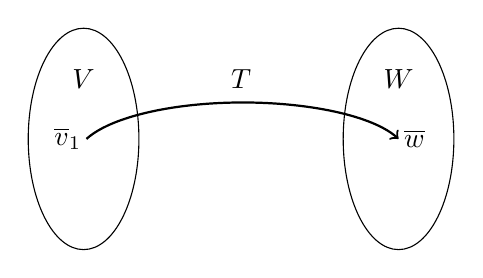
\begin{tikzpicture}
        \draw (2,0) ellipse (20pt and 40pt);
        \draw[] (-2,0) ellipse (20pt and 40pt);
        \draw[<-, thick] (2,0) arc (20:160: 60pt and 20pt);
        \draw (0,1)  node[anchor = north] {$T$};
        \draw (2,1)  node[anchor = north] {$W$}; 
        \draw (-2,1) node[anchor = north] {$V$};
        \draw (-2.2,0) node {$\bar v_1$};
        \draw (2.2,0) node {$\bar w$};
    \end{tikzpicture}
\end{center}

Suppose $V$ and $W$ are two linear spaces over $\b F$. $T$ is a function with domain $V$ and codomain $W$. $T$ is called linear iff 
\begin{enumerate}
    \item $T(\bar v_1 + \bar v_2) = T(\bar v_1) + T(\bar v_2)$
    \item $T(\lambda \bar v) = \lambda \cdot T(\bar v)$
\end{enumerate}
$\forall \bar{v}_1, \bar{v}_2 \in V$ and $\forall \bar{v} \in V, \forall \lambda v \in \b F$.
\begin{example}
    Let $V = \b R^3, W = \b R^4$. Define $T$ as $(x_1, x_2, x_3) \mapsto (x_1,0,0,0)$
\end{example}
\begin{example}
    $T: \c P(x) \to \c P(x)$, where $\displaystyle f(x) \mapsto \int_{10}^x f(x) \ dx$ is a linear map.
\end{example}
\begin{definition}
    $\c L\{V, W\}$ denotes the set of all linear maps from $V$ to $W$. Note that $\c L\{V, W\}$ with $+$ and $\cdot$ becomes a vector space over $\b F$. This requires the additions of functions and multiplications of linear maps by scalars (from $\b F$). Given $T_1, T_2 \in \c L(V,W)$ we define addition as $(T_1 + T_2)(\bar v) := T_1(\bar v) + T_2(\bar v)$, multiplication as $(\lambda T)(\bar v) : = \lambda \cdot T(\bar v)$. 
\end{definition}
\begin{theorem}
    In finite vector space $V,W$, let $\li{\bar v}n$ be a basis for $V$, let $\li{\bar w}m$ be any vectors in $W$. Then there exist a unique linear map $T \in \c L \lb V, W \rb$ such that $T(\bar v_j) = \bar w_j \forall j$.
\end{theorem}
\begin{proof}
    Any vector in $V$ has a unique representation $\alpha_1 \bar v_1 + \alpha_2\bar v_2 + \cdots + \alpha_n \bar v_n = \bar v$.  \\ Define $T(\bar v):= \underbrace{\lincomb \alpha {T(\bar v)}n}_{\in W}$ This makes $T$ a linear map from $V$ to $W$. Indeed if $\lambda \in \b F$, then $T(\lambda \bar v) = T(\sum_{j = 1}^n \lambda \alpha_j \bar v_j) = \lambda \sum_{j = 1}^n \alpha_j \bar wj$. Suppose $\tilde T(\bar v_j) = \bar w_j$ for all $j$, then $T = \tilde T$ as a map function by linearity and basis.
\end{proof}
\begin{theorem}
    Let $\nul (T):= \lb \bar v \in  v : T(\bar v) = 0 \rb$. $\nul (T)$ is a subspace of $V$.
\end{theorem}
\begin{theorem}
    Let $\range (T):= \lb \bar w \in W : T(\bar v) = \bar w \rb$. $\range(T)$ is a subspace of $W$.
\end{theorem}
\begin{proof}
    The proof is trivial and is left as an exercise for the reader .
\end{proof}
\begin{example}
    Let $T: f \to f', V:= \c P(x), W:= \c P(x)$. $\nul(T) = \c P_0(x)$, $\range(T) = \c P_2(x)$. \\
    Let $T: f \to f'', V:= \c P(x), W:= \c P(x)$. $\nul(T) = \c P_0(x)$, $\range(T) = \c P_1(x)$.
\end{example}

 \vfill
%\section{Polynomials}
Recall we call consider polynomials over $\b C$ or $\b R$.
\begin{theorem}
    For any $z_1, z_2 \in \b C$, we define $|z|  = \sqrt{a^2 + b^2}$, we know that 
    \begin{enumerate}
        \item $|z_1 \cdot z_2| = |z_1| \cdot |z_2|$
        \item $|z_1 \cdot z_2| \leq |z_1| + |z_2|$
    \end{enumerate}
\end{theorem}
\begin{proof}
Left as an execise.
\end{proof}
\subsection{Axler's Recap on Polynomial}
\begin{theorem}
    Suppose $p(x) \in \c P(\b F)$, is identically zero. Then all of its coefficient must be $0$. 
\end{theorem}
\begin{proof}
    If $p(x) = a_0 + a_1x + \cdots + a_nx^n$, then $a_j = \frac{p^{(j0}(0)}{j!}$, If $p(x) \equiv 0$, then $p^{(j)}(x) = 0$, so $a_j = \frac{0}{j!} = 0 \forall j$
\end{proof}
\begin{corollary}
    Suppose $p(x) \equiv q(x)$ for $p,q \in \c P(\b F)$, then all coefficients of $p$ are the same as all coefficients of $q$.
\end{corollary}
\subsection{Zero of polynomials and their algebraic manifestations}
\begin{algorithm}[Euclidean Algorithm for polynomials]
 Given $p(x), s(x)$, without the loss of generality, $\deg p(x) > \deg s(x)$, otherwise it's boring; we can always find $q(x), r(x)$ such that $p(x) = s(x)q(x) + r(x)$, where $\deg r(x) < \deg s(x)$.
\end{algorithm}
\begin{corollary}
    $p(a) \iff p(x) = (x - a)q(x)$ for some $a \in \b F$.
\end{corollary}
\begin{proof}
    If $p(a) = (x-a)q(x)$, then $p(a) = 0 \cdot q(a) = 0$. \\
    Conversely, suppose $p(a) = 0$, by division algorithm we have $p(x) = (x - a)q(x) + r(x)$, where $\deg r \leq \deg (x-a)$, therefore $r(x) = c$ for some $c \in \b F$. Plug in $a$ and we get $(a - a)q(a) + c = 0 \implies 0 + c = 0 \implies c = 0$. Therefore $p(x) = (r-a)q(x)$.
\end{proof}
\begin{theorem}
    Let $p(x)$ be a nonzero polynomial with coefficients in $\b F$ have degree $n$. Then $p$ has at most $n$ zeros in $\b F$.
\end{theorem}

\begin{proof} $ $ \\
    \textit{Base case:} $\deg p = 1$, i.e. $p(x) = a_1x + a_0$ for some $a_1 \in \b F^\times, a_0 \in \b F$. Then $p\left(\frac{-b}{a}\right) = 0$, so $p$ has exactly one zero. \\
    \textit{Inductive Hypothesis:} Suppose the statement is true for all polynomials for all polynomials of degree less than $m$. \\
    \textit{Inductive Step:} Take $p(x)$ to be a degree $m$ polynomial. If $p$ has no zeros in $\b F$, we are done. If $p$ has a zero, by corollary we have $p(x) = (x - a)q(x)$, where $\deg q = m - 1$. So the inductive hypothesis applies and $q$ at most $n-1$ distinct zeros in $\b F$.
\end{proof}
\begin{theorem}[Fundamental Theorem of Algebra]
    Every nonconstant polynomial with complex coefficients has a zero.
\end{theorem}
\begin{proof}[Proof with ``Black Box" from Complex Analysis] $ $ \\
    Assume $\deg p \geq 1$. Assume that $p(a) \neq 0 \ \forall a \in \b C$. Consider the function $\frac{1}{p(x)}$ is well-defined $\forall x \in \b C$ and is analytic in $\b C$, more over $\lim_{|z| \to \infty} \frac{1}{p(z)} = 0$. We know that 
    \begin{align*}
        p(x) &= a_0 + a_1 x + \cdots + a_n x^n \\
        &= x^n \left( \frac{a_0}{x^n} + \frac{a_1}{x^{n-1}} + \cdots + a_n\right) \\
        \frac{1}{p(x)} &= \frac{1}{x^n \left( \frac{a_0}{x^n} + \frac{a_1}{x^{n-1}} + \cdots + a_n\right)} 
    \end{align*}
    As $\displaystyle |x| \to \infty, \displaystyle \frac{1}{x^n} \to 0$. Since $\displaystyle \left|\frac{1}{x^n}\right| = \frac{1}{|x|^n} \to 0$. But $\displaystyle \frac{a_0}{x^n} + \frac{a_1}{x^{n-1}} + \cdots + a_n \to a_n \neq 0$. Hence $\displaystyle \frac{1}{p(x)} \to 0$ as $|x| \to -\infty$. \\
    By Louisville's theorem, any analytic function with this property has to be constant. But $\frac{1}{p(x)}$ is non-constant, so $p$ must have at least $1$ zero in $\b C$.
\end{proof}
\begin{corollary}
    Any polynomial $p(x)$ with coefficients in $\b C$ factors as follows 
    \[ p(x) = c(x - a_1)(x - a_2) \cdots (x - a_m), c \neq 0\]
\end{corollary}
\begin{proof}
    By Induction it's clear for degree $1$ and if $\deg p = m$ then factor $p(x) = (x - a)q(x)$ and repeat the process for $q$.
\end{proof}
\begin{question}
    What happens over $\b R$?
\end{question}
\begin{theorem}
    If $p(x)$ has coefficient in $\b R$, and $c \in \b C$ is a zero of $p$, then $\bar c$ is also a zero of $p$.
\end{theorem}
\begin{proof}
    $p(c) = 0$ means \[a_0 + a_1 c + a_2 c^2 + \cdots + a_nc^n = 0\] We then can see \begin{align*}
        \bar{a_0} + \bar{a_1 c} + \bar{a_2 c^2} + \cdots + \bar{a_n c^n} &= \bar 0 = 0 \\
        \bar{a_0} + \bar{a_1} \bar{c} + \bar{a_2} \bar{c^2} + \cdots + \bar{a_n} \bar{c^n} & = 0 \\
        a_0 + a_1 \bar c + a_2 \bar{c^2} + \cdots + a_n \bar{c^n} &= 0
    \end{align*}
    Hence $p(\bar c) = 0$ as well.
\end{proof}
So over $\b C$, a polynomial with real coefficient factors as follows
\[ p(x) = (x - a_1)(x - a_2)\cdots(x - a_n)(x - \lambda_1)(x - \bar{\lambda_1})(x - \lambda_2)(x - \bar{\lambda_2}) \cdots (x - \lambda_m)(x - \bar{\lambda_m})\]
For some $c \in \b R, \li an \in \b R, \li \lambda m \in \b C$. \\
To translate this into a factorization over $\b R$, we can see that $x^2 - (\lambda + \bar \lambda) + |\lambda|^2$. These are quadratic with $\Delta < 0$. Indeed, 
\[ (\lambda + \bar \lambda)^2 - 4 |\lambda|^2 = \lambda ^2 - 2 |\lambda |^2 + {\bar \lambda}^2 = 2 \text{Re} \lambda^2 - 2 |\lambda|^2 \]
Notice that $\text{Re} \lambda^2 \leq |\lambda|^2$ and $\text{Re} \lambda^2 = |\lambda|^2$ iff $\lambda \in \b R$, therefore $\Delta < 0$.
\begin{question}
    Why do we study polynomials?
\end{question}
\begin{answer} $ $
\begin{enumerate}
    \item We will form polynomials in linear operators
    \item We will associate special polynomials with linear operators.
\end{enumerate}
\end{answer}
\begin{remark}
An operator has he same co-domain as its domain.
\end{remark}

 \vfill
%\section{Eigenvalues, Eigenvectors, and
Invariant Subspaces}
\subsection{Invariant Subspaces}
\begin{definition}
    Let $T \in \c L(V,V)$ on a vector space $V \neq \lb 0 \rb$. A subspace $U \subseteq V$ is called an invariant subspace is invariant under $T$ if $Tu \in U \ \forall u \in U$.
\end{definition}
\begin{example}
    For any $T \in \c L(V,V)$, the following subspaces are invariant:
    \begin{enumerate}
        \item $\lb 0 \rb$
        \item $V$
        \item $\nul T = \lb v \in V : Tv = 0 \rb$ \\
        If $Tv \in \nul T$, then $Tv = 0 \in \nul T$.
        \item $\range T = \lb w \in W : w = Tv \text{ for some } v \in V \rb$ \\
        So $Tw \in \range T$.
    \end{enumerate}
\end{example}
\begin{question}
    What are $1$-dimensional invariant subspaces?  
\end{question}
\begin{answer}
Then $U = \spa(u)$ for some $u \neq 0$. Invariant means $Tu = \lambda u$ for some $\lambda \in  \b F$, where $u$ is the eigenvector of $T$ and $\lambda$ is the eigenvalues.
\end{answer}
\begin{remark}
    $u \neq 0$ if $u$ is a eigenvector is $T$. $\lambda = 0$ is possible.
\end{remark}
\begin{proposition} Let $T$ be a linear operator in $V$, then the following are equivalent
\begin{enumerate}
    \item $\lambda$ is a eigenvalue of $T$.
    \item $T - \lambda\b I$ is not invertible.
    \item $T - \lambda \b I$ is not injective.
    \item $T - \lambda \b I$ is not surjective.
\end{enumerate}
\end{proposition}
We have already proven that statement $2,3,4$ are logically equivalent. 
\begin{theorem}
    Suppose $\li vm$ are eigenvectors of $T \in \c L(V)$ corresponding to distinct eigenvalues $\li \lambda m$ will be linearly independent.
\end{theorem}
\begin{proof}
Suppose $\li vm$ are linearly independent. By linear dependence lemma, we find a the minimum index $k \leq m$ such that $v_k \in \spa (\li v{k-1})$. i.e.
\begin{equation} \label{eqn1}
     v_k = \lincomb{\alpha}{v}{k-1} 
\end{equation}
Apply linear transformation on both sides 
\begin{equation} \label{eqn2}
    Tv_k = T\lincomb{\alpha}{v}{k-1} 
\end{equation}
\begin{equation} \label{eqn3}
    \lambda v_k = \alpha_1 \lambda_1 v_1 + \alpha_2 \lambda_2 v_2 + \cdots + \alpha_n \lambda_n v_n 
\end{equation} 
We multiply by equation \ref{eqn1} by $\lambda_m$ and subtract by from \ref{eqn3} and we get \[ 0 = \alpha_1 (\lambda_1 - \lambda_k)v_1 + \alpha_2(\lambda_2 - \lambda_k)v_2 + \cdots + \alpha_{k-1} (\lambda_{k-1} - \lambda_k)v_{k-1}\]
A contradiction since $k$ is not the minimum index with the property chosen above. Therefore the list $\li vm$ must be linearly independent.
\end{proof}
\begin{corollary}
An operator $T \in \c L(V)$ has at most $\boxed{\dim V}$ distinct eigenvalues.
\end{corollary}
\subsection{Eigenvectors and Upper-Triangular
Matrices}
\subsubsection{Polynomials in T}
\begin{definition}
    Suppose $T \in \c L(V)$, then $T^k$ is defined as
    \[ T^k := \underbrace{k \circ k \circ \cdots \circ k}_{k \text{ times}}\]
    Notice that $T^0 = \b I, T^1 = T$.
\end{definition}
\begin{definition}
    If $p(x) = a_0 + a_1x + \cdots + a_nx^n$, then we can define $p(T)$ as $a_o\b I + a_1T + a_2T + \cdots + a_nT^n$.
\end{definition}
\begin{example}
    Let $V := \c P(\b R), S: p \mapsto 3p'' +  2p' + p, D: p \mapsto p'$. We can see that $S$ can be expressed as $S = D^0 + 2D + 3D^2$. Therefore \[\c M(S) = 3\c M^2(D) + 2\c M(D) + M(\b I)\] we need to have to take the same basis for inputs and output when forming $\c M(\cdot)$.  
    
    \noindent Let's use our favorite basis $1,x,x^2, x^3$. We then can see
    \[ \c M(D) = \bml 0 & 1 & 0 & 0 \\ 0 & 0 & 2 & 0 \\ 0 & 0 & 3 & 0 \\ 0 & 0 & 0 & 0 \bmr, \c M(S) = \bml 1 & 2 & 6 & 0\\ 0 & 1 & 4 & 18\\ 0 & 0 & 1 & 6 \\ 0 & 0 & 0 & 1 \bmr\]
\end{example}
\begin{question}
    What is the best matrix representation for an operator?
\end{question}
\begin{question}
    What information about eigenvalues/eigenvectors can be read off from a matrix representation?
\end{question}
\begin{theorem}
    Suppose $T \in \c L(V)$ and $\li vn$ is a basis of $V$. Then the following are logically equivalent:
    \begin{enumerate}
        \item  $\c M(T)$ is upper triangular.
        \item $Tv_j \in \spa (\li vj)$ $\forall j = 1,2, \ldots, n$.
        \item $\spa (\li vj)$ is invariant under $T$ $\forall j = 1,2,\ldots, n$.
    \end{enumerate}
\end{theorem}
\begin{proof}
    $1) \implies 2) $ \[\bml * & * & * & * & \cdots & * \\  & * & * & * & \cdots & * \\  &  & * & * & \cdots & * \\ & & & * & \cdots & * \\  & & & & \ddots & \vdots \\  & & & & & * \bmr\] We can see that $2)$ holds true by inspection. \\
    $2) \implies 3)$ Consider $Tv_h$ for $h \leq j$, by $2)$ we have $Tv_k \in \spa(\li vh) \subseteq \spa (\li vj)$. So $\spa (\li vj)$ is invariant under $T$. \\
    $3) \implies 2)$ Consider $Tv_j$, by $3)$ it is a linear combination of $\li vj$ because $Tv_j \in \spa(\li vj)$ so $\c M(T)(i,j) = 0$ if $i > j$.
\end{proof}
\begin{question}
    What about conditions for lower-triangular matrices?
\end{question}
\begin{theorem}
    Over $\b C$ every linear operator has an upper-triangular matrix representation.
\end{theorem}
\begin{lemma}
Over $\b C$, every linear operator has at least one eigenvalue.
\end{lemma}
\begin{proof}
    Take $v \in V\ \backslash \lb 0 \rb$, and consider the list $v, Tv, T^2v, \ldots, T^nv$ where $n = \dim V$. There is a nontrivial linear combination of these vectors which is $0$. Suppose the equation \[a_0v_1 + a_1Tv + a_2T^2v + \cdots + a_nT^nv = 0\]
    i.e. $p(T)v = 0$ for nonconstant $p(x) : = a_0 + a_1x + a_2x^2 + \cdots + a_nx^n$. By the fundamental theorem of algebra $p$ splits into linear factors over $\b C$.
    \[ p(x) = c(x - \lambda_1)(x - \lambda_2) \cdots (x - \lambda_m)\] for some $m \leq n$. Therefore 
    \[ p(T)v = c(T - \lambda_1 \b I)(T - \lambda_2  \b I) \cdots (T - \lambda_m \b I)\]
    Therefore at least one of these factors is not injective. This shows that $T$ has at least $1$ eigenvalue.
\end{proof}











 \vfill
%%!TEX root = ./main.tex
\section{Inner Product Spaces}
\subsubsection*{Motivation}
\begin{definition}
    In $\b R^n$, the dot product of $\vec x$ and $\vec y$ is defined by  
\[ \vec x \cdot \vec y := x_1y_1 + x_2y_2 + \cdots + x_ny_n\]
for $\vec x = (\li xn), \vec y = (\li yn)$.
\end{definition}
\subsection{Inner Product and Norms}
\subsubsection*{Settings}
$V$ is a vector space over $\b F$, we can define the following mapping $ \la \ast, \ast \ra : V \times V \to \b F$.
\begin{definition}
$\la \cdot, \cdot \ra$ is called an inner product if it satisfying the following rules:
\begin{enumerate}
    \item(additivity in the first slot) $\la \vec v + \vec u, \vec w \ra = \la \vec v + \vec w \ra + \la \vec u, \vec w \ra, \ \forall \vec v, \vec u, \vec w \in V$
    \item(homogeneity in the first slot) $\la \lambda \vec v, \vec w \ra = \lambda \la \vec v + \vec w \ra, \ \forall \vec v \vec u, \vec w \in V, \lambda \in \b F$
    \item(conjugate symmetry) $\la \vec v, \vec w \ra = \overline{\la \vec w, \vec v \ra}, \ \forall \vec v,\vec w \in V$
    \item(positivity) $\la \vec v, \vec v \ra \geq 0, \ \forall \vec v \in V$
    \item(definiteness) $\la \vec v, \vec v \ra = 0$ iff $\vec v = \vec 0$.
\end{enumerate}
\end{definition}
\begin{question}
What about linearity in the second slot?
\end{question}
\begin{answer} We can compute
\[ \la \vec v, \vec u + \vec w \ra = \overline{\la \vec u + \vec w, \vec v\ra} = \overline{\la \vec u, \vec v \ra + \la \vec w, \vec v \ra} = \overline{\la \vec u, \vec v \ra} + \overline{\la \vec w, \vec v\ra } = \la \vec v, \vec u\ra + \la \vec v, \vec w\ra\]
\[ \la \vec v, \lambda \vec u\ra = \overline{\la \lambda \vec u, \vec v\ra} = \overline{\lambda \la \vec u,\vec v\ra} = \bar \lambda \ \overline{\la \vec u, \vec v\ra} = \bar \lambda \la \vec v, \vec u \ra\]
Not quite. \frownie{}
\end{answer}
\begin{remark}
    If $\vec v \in V$ is fixed then the function $\la \ast, \vec v \ra : \vec u \mapsto \la \vec u, \vec v \ra$ is a function functional. 
\end{remark}
\begin{example}
    On $\b R^n$, we could use any function of the type
    \[ c_1x_1y_1 + c_2x_2y_2 + \cdots + c_nx_ny_n\] where all $c_j \in \b R^+$.
\end{example}
\begin{remark}[Generalization to $\b C^n$]
    The inner product of this form of the standard product to $\b C^n$ can be defined as
    \[ \la \vec x, \vec y \ra = x_1\bar y_1 + x_2\bar y_2 + \cdots + x_n\bar y_n\]
\end{remark}
\begin{remark}[Generalization to any function space]
    \[ \la f, g \ra : = \int_D f(t)\overline{g(t)} dt\]
    or generally \[ \la f, g \ra : = \int_D f(t)\overline{g(t)}w(t) dt\]
    where $w(t)$ is the positive weight function. e.g. if $V = \c P(\b R)$, or $V = \c P(\b C)$, then 
    \[ \la f, g \ra : = \int_0^\infty f(t)\overline{g(t)}e^{-t} dt\]
\end{remark}
\begin{definition}
    For $\vec v \in V$, the (Euclidean) Norm is defined as
    \[ ||\vec v|| : = \sqrt{\la \vec v,\vec v \ra}\] 
\end{definition}
\begin{theorem}(Properties of Norms)
    \begin{enumerate}
        \item $||\lambda \vec v || = |\lambda| \ ||v|| \ \forall v \in V, \forall \lambda \in \b F $
        \item $||\vec v|| > 0$ for all $v \in V$
        \item $||\vec v|| = 0$ if and only if $v = 0$ 
    \end{enumerate}
\end{theorem}
\begin{definition}
    An inner product space is a vector space $V$ along with and inner product on $V$.
\end{definition}
\begin{definition}
    For $u,v \in V$, we say $\vec u$ and $\vec v$ is orthogonal if $\la \vec u, \vec v\ra = 0$
\end{definition}
\begin{theorem}[Pythagorean Theorem] $ $
\begin{center}
    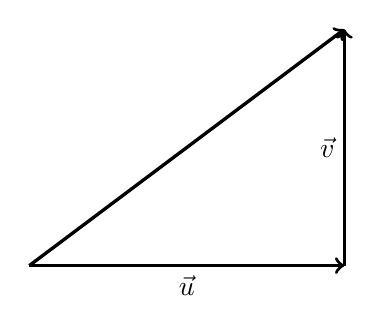
\begin{tikzpicture}
        \draw[->, very thick] (4,0) -- (4,3);
        \draw[->, very thick] (0,0) -- (4,0);
        \draw[->, very thick] (0,0) -- (4,3);
        \draw (2,0) node[anchor = north] {$\vec u$};
        \draw (4,1.5) node[anchor = east] {$\vec v$};
    \end{tikzpicture}
\end{center}
\[ ||\vec u + \vec v||^2 = ||\vec u||^2 + ||\vec v||^2 \iff \la \vec u + \vec v, \vec u + \vec v\ra = \la \vec u, \vec u \ra + \la \vec v, \vec v \ra \]
\end{theorem}
\begin{proof} We compute
    \[ \la \vec u + \vec v, \vec u + \vec v\ra = \la \vec u,\vec u \ra + \la \vec u , \vec v \ra + \la \vec v, \vec u \ra + \la \vec v,\vec v \ra = \la \vec u,\vec u \ra + 0 + 0 + \la \vec v,\vec v \ra = ||\vec u|| + ||\vec v|| \]
\end{proof}
\subsubsection*{Obeservation}
Given $\vec u,\vec v \in V$ such that $\vec v \neq 0$, we want to modify $\vec u$ such that $\vec u + c\vec v$ is orthogonal to $\vec v$. We know that $\la \vec v + c\vec v, \vec v \ra = 0$, solve for $c$ gives $c = \displaystyle\frac{-\la \vec u, \vec v\ra}{\la \vec v, \vec v \ra}$.
\begin{center}
    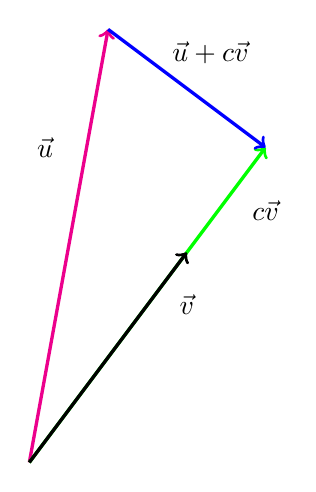
\begin{tikzpicture}
        \draw[->, very thick, color = magenta] (0,0) -- (1, 5.5);
        \draw[->, very thick, color = green] (0,0) -- (3, 4);
        \draw[->, very thick] (0,0) -- (2,2.66666666);
        \draw[->, very thick, color = blue] (1, 5.5) -- (3,4);
        \draw (2,2) node {$\vec v$};
        \draw (0.2,4) node {$\vec u$};
        \draw (3,3.2) node {$c\vec v$};
        \draw (2.3, 5.2) node {$\vec u + c\vec v$};
    \end{tikzpicture} 

    An orthogonal decompostion
\end{center}
\begin{theorem}[Cauchy-Schwarz Inequality]
    For any $u,v \in V$ where $V$ is a inner product space, the following holds
    \[ |\la \vec u,\vec v \ra| \leq ||\vec u|| \cdot ||\vec v||\]
\end{theorem}
\begin{proof}
    Given $u,v \in V$, we can assume without the loss of generality that $v \neq 0$. So we can consider vectors $u + cv$ and $v$ that are orthogonal for the choice that 
    \[ c: = \frac{ - \la u,v \ra}{\la v,v\ra}\]
    By Pathgrathrean theorem, $||u + cv||^2 + ||cv||^2 = ||u||^2$. But $||cv||^2 = |c|^2||v||^2$ and recall \[ c= \frac{- \la u,v\ra}{\la v,v\ra}, \text{ so } c^2= \frac{|\la u,v\ra|^2}{\la v,v\ra^2} = \frac{|\la u, v \ra|^2}{||v||^4}, \text{ therefore } ||cv||^2 = \frac{|\la u, v \ra|^2}{||v||^4} ||v||^2 = \frac{|\la u, v \ra|^2}{||v||^2}\]
    So by dropping $|| u + cv||^2 > 0$, we obtain $||cv||^2 \leq ||u||$, i.e, 
    \[ \frac{|\la u, v \ra|^2}{||v||^2} \leq ||u||^2 \implies |\la u,v\ra|^2 \leq ||u|^2 \cdot ||v||^2 \implies |\la u,v \ra|^2 \leq ||u|| \cdot ||v||\]
\end{proof}
\begin{theorem}[Triangle Inequality]
\[ ||\mathbf u + \mathbf v|| \leq ||\mathbf u|| + ||\mathbf v||\]
\end{theorem}
\begin{proof}
We want to show
\[ ||\mathbf u + \mathbf v|| \leq \left( || \mathbf u || + ||\mathbf v||\right)^2\]
We can factor them out 
\[ \la \mathbf u, \mathbf u \ra + \la \mathbf u, \mathbf v \ra + \la \mathbf v, \mathbf u \ra + \la \mathbf v, \mathbf v \ra \leq ||\mathbf u||^2 + 2 ||\mathbf u|| \cdot ||\mathbf v|| + ||\mathbf v||^2\]
\[ 2\Re \la \vec u, \vec v \ra \leq 2||\vec u||\cdot ||\vec v|| \]
%\begin{center}
%    \begin{tikzpicture}
%        \draw[->, thick] (0,0) -- (6,2);
%        \draw[->, thick] (0,0) -- (6,0);
%        \draw (3,0) node[anchor = north] {$\Re v$};
%        \draw (3,1) node[anchor = north] {$v$};
%    \end{tikzpicture}
%\end{center}
\end{proof}
\begin{theorem}[Alternative Version of Triangle Inequality]
    \[ \big| ||\vec u|| - ||\vec v|| \big| \leq ||\vec u - \vec v||\]
\end{theorem}
\begin{proof}
    Notice that 
    \[   ||\vec u|| - ||\vec v|| \leq ||\vec u - \vec v|| \iff ||\vec u|| \leq ||\vec u - \vec v||  + ||\vec v||\]
    Which is the triangle inequaliy. Swapping out $\vec u$ and $\vec v$ gives us \[   ||\vec v|| - ||\vec u|| \leq ||\vec v - \vec u|| \iff ||\vec u|| \leq ||\vec u - \vec v||  + ||\vec v||\]
    Combining these equations gives us
    \[ \big| ||\vec u|| - ||\vec v|| \big| \leq ||\vec u - \vec v||\]
\end{proof}
\begin{fact}[Fun inequalities]
\[ ||\vec u + \vec v||^2 + ||\vec u + \vec v||^2 = 2\left(||\vec u||^2 + ||\vec v||^2\right)\]
\end{fact}
\subsection{Orthogonality}
\begin{definition}
    A list $\li{\vec v}{k}$ is $V$ is called orthonormal if \[ \la \vec v_i \vec v_j \ra = \delta_{ij} = \left\{\begin{array}{cc}
        1 & \text{if } i = j \\
        0 & \text{if } i \neq j \\
    \end{array} \right.\]
\end{definition}
\begin{lemma}
    Any list of orthonormal vectors is necessarily linearly indepedent.
\end{lemma}
\begin{proof}
    Suppose $\lincomb{\alpha}{\vec v}{k} = \vec 0$. We can compute on the standard inner product
    \[ \la \lincomb{\alpha}{\vec v}{k} , \vec v_1 \ra = \alpha_1 \la \vec v_1, \vec v_1 \ra + \alpha_2 \la \vec v_2, \vec v_1 \ra + \cdots + \alpha_k \la \vec v_k, \vec v_1 \ra \implies \alpha_1 = 0\]
    \[ \la \lincomb{\alpha}{\vec v}{k} , \vec v_2 \ra = \alpha_1 \la \vec v_2, \vec v_2 \ra + \alpha_2 \la \vec v_2, \vec v_2 \ra + \cdots + \alpha_k \la \vec v_k, \vec v_2 \ra \implies \alpha_1 = 0\]
    \[ \vdots \]
    \[ \la \lincomb{\alpha}{\vec v}{k} , \vec v_k \ra = \alpha_1 \la \vec v_1, \vec v_k \ra + \alpha_2 \la \vec v_2, \vec v_k \ra + \cdots + \alpha_k \la \vec v_k, \vec v_k \ra \implies \alpha_k = 0\]
    Hence $\li{\vec v}k$ is linearly indepedent.
\end{proof}
\begin{question}
    What is nice about orthonormal basis?
\end{question}
\begin{answer}
    If $(\li{\vec v}n)$ is an orthonormal basis, then an arbitary vector can be written as 
    \[ \vec v = \la \vec v, \vec v_1 \ra \vec v_1 + \la \vec v, \vec v_2 \ra \vec v_2 + \cdots + \la \vec v, \vec v_n \ra \vec v_n\]
    Furthermore, we can conclude the following theorem:
\end{answer}
\begin{theorem}[Generalized Pythagorean Theorem]
\[ ||\vec v||^2 = \sum_{j = 1}^{n} \big| \la \vec v, \vec v_j \ra \big|^2\]
\end{theorem}
\begin{algorithm}[Gram-Schmidt Algorithm]
    \texttt{Input}: Any $\li{\vec v}m$ that is linearly independent. \\
    \texttt{Output}: $\li{\vec e}m$ such that $\vec e_j \in \spa (\li{\vec v}j)$ for all $j \leq n$.
    \begin{proof}[Process] $ $
        \begin{align*}\vec e_1 &= \frac{\vec v_1}{||\vec v_1||} \\
        \vec e_2 &= \frac{\vec v_2 - \la \vec v_2, \vec e_1 \ra \vec e_1}{||\vec v_2 - \la \vec v_2, \vec e_1 \ra \vec e_1||} \\
        \vec e_3 &= \frac{\vec v_3 - \la \vec v_3, \vec e_1 \ra \vec e_1 - \la \vec v_3, \vec e_2 \ra \vec e_2}{||\vec v_3 - \la \vec v_3, \vec e_1 \ra \vec e_1 - \la \vec v_3, \vec e_2 \ra \vec e_2||} \\
        \vdots \\
        \vec e_n &= \frac{\vec v_n - \la \vec v_{n}, \vec e_1 \ra \vec e_1 - \la \vec v_n, \vec e_2 \ra \vec e_n \cdots - \la \vec v_n - \vec e_{n-1} \ra \vec e_{n-1}}{||\vec v_n - \la \vec v_{n}, \vec e_1 \ra \vec e_1 - \la \vec v_n, \vec e_2 \ra \vec e_n \cdots - \la \vec v_n - \vec e_{n-1} \ra \vec e_{n-1}||}
        \end{align*}
    \end{proof}
\end{algorithm}
\begin{remark}[Projection orthonal with the repect to inner product]
    Given a subsace $U$ of $V$ for finie dimensioanl vector space $V$, there is a projector $P_V$ that project all vectors in $V$ on $V$ orthogonally.
\end{remark}
\begin{remark}[Relations between inner product and linear functionals]
    Suppose $V$ is finite dimensional vector space. Given any $\vec u \in V$, then function $\la \cdot, \vec u\ra$ is a linear functional (i.e. an element of $V' = \c L(V,\b F)$)
\end{remark}
\begin{theorem}[Riesz Representation Theorem]
    For any $\varphi \in V'$ there exists $\vec v \in V$ such that $\la \vec v, \vec v \ra = \varphi (\vec v)$ for al $\vec v \in V$.
\end{theorem}
\begin{proof}
    Left as an exercise.
\end{proof} \vfill
%%!TEX root = ./main.tex
\section{Operators on Inner Product Spaces}
\subsection{Self-Adjoint and Normal Operators}
\begin{definition}
	Suppose $T \in L(V,W)$, we define $T*$ by this formula 
	\[ \la T\vec v, \vec w \ra_W = \la \vec v, T^* \vec w \ra_V\]
\end{definition}
We can think og $\vec w$ as fixed, we note that $\la T \ast, \vec w \ra$ is a linear functiona;. hence it has a representer by Riesz, so we are entitled to call it $T^*\vec w$ such that 
\[ \la T\vec v, \vec w \ra = \la \vec v, T^* \vec w \ra \]
Hence we have $T^* \in \c L(W,V)$. We want to verify this property. Consider $T*(\vec w_1 + \lambda \vec w_2)$. We compute 
\begin{align*}
	\la \vec v, T*(\vec w_1 + \lambda \vec w_2) \ra &= \la T\vec v, \vec w_1 + \lambda \vec w_2\ra \\
	&= \la T\vec v, \vec w_1 \ra + \bar \lambda \la T\vec v + \vec w_2 \ra \\
	&= \la \vec v, T^*\vec w_1 \ra +  \bar \lambda \la \vec v, T^* \vec w_2 \ra \\
	&= \la \vec v, T^*\vec w_1 \ra +   \la \vec v, \lambda T^* \vec w_2 \ra \\
	&= \la \vec v, T^*\vec w_1 +  \lambda T^*w_2 \ \ra \forall \vec v \in V, \vec w_1, \vec w_2 \in W, \lambda \in \b F 
\end{align*}
So $T^*(\vec w_1 + \lambda \vec w_2) = T^* \vec w_1 + \lambda T^* \vec w_2$.

\begin{theorem}[Properties of the adjoint]
Let $T \in \c L(V,W)$, we have
	\begin{enumerate}
		\item $(S + T)^* = S^* + T^*$
		\item $(\lambda T)^* = \bar \lambda T^*$
		\item $(S \cdot T)^* = T^*S^*$
		\item $(\lambda T)^* = \bar \lambda T^*$
		\item $\b I^* = \b I$
	\end{enumerate}
\end{theorem}
\begin{proof} Refer to book page 206
\end{proof}
\begin{theorem}[Null space and range of adjoint]
Let $T \in \c L(V,W)$, then
	\begin{enumerate}
		\item $\nul T^* = (\range T)^\perp$
		\item $\range T^* = (\nul T)^\perp$
		\item $\nul T = (\range T*)^\perp$
		\item $\range T = (\nul T^*)^\perp$
	\end{enumerate}
\end{theorem}
\begin{proof}
Let $\vec w \in W$. Then 
\begin{align*}
	\vec w \in \nul T^* &\iff T^* \vec w = 0 \\
	&\iff \la \vec v, T^* \vec w \ra = 0 \ \forall \vec v \in V \\
	&\iff \la T\vec v, \vec w \ra \ \forall \vec v \in V \\
	&\iff \vec w \in (\range T)^\perp
\end{align*}
(b),(c),(d) follows by a similar logic and is left as an exercise.
\end{proof}

\begin{definition}
Let $T \in \c L(V)$. $T$ is called self-adjoint if $T^* = T$.
\end{definition}
\begin{definition}
	$T$ is called normal if $TT^* = T^*T$.
\end{definition}
%\begin{example}
%	Let $V$ be $\b R^3$ with the standard inner product, let $T \in \c L(V)$ such that $T: (x_1,x_2,x_3) \mapsto (x_1,2x_2,3x_3)$.
%\end{example}
\begin{example}
	Suppose $T \in \c L(V)$, we can define $T: \vec v \mapsto \la \vec , \vec x \ra \vec y$ for some fixed $\vec x, \vec y$ in $V$. Compute $T^*$. \\
	We compute 
	\begin{align*}
		\langle \vec v, T^* \vec w \rangle &= \langle T \vec v, \vec w \rangle  \\
		&= \langle \langle \vec v, \vec x \rangle \vec y, \vec w \rangle  \\
		&= \langle \vec v, \vec x \rangle \langle \vec y, \vec w \rangle \\
		 &= \langle \vec v, \overline{\langle \vec y, \vec w \rangle} \vec x \rangle \\
		 &= \langle \vec v, \langle \vec w, \vec y \rangle \vec x \rangle
	\end{align*}
	hence we can concldue $T^* \vec w = \la \vec w, \vec y \ra \vec x$ for all $\vec w \in W$.
\end{example}
\newpage
\subsubsection{Matrix representation}
Suppose $T \in \c L(V,W)$, where $V,W$ are finite-dimensional vector spaces. Let $\li{\vec e}n$ be an orthonormal basis for $V$ and $\li{\vec f}m$ be a orthonormal basis for $W$. We can see that $\c M(T)$ is obtained through
\[ T \vec e_j = \la T\vec e_j, \vec f_1 \ra \vec f_1 + \la T\vec e_j, \vec f_2 \ra \vec f_2 + \cdots + \la T\vec e_j, \vec f_m \ra \vec f_m\]
\[ T^* \vec f_k = \la T^* \vec f_k, \vec e_1 \ra \vec e_1 + \la T^* \vec f_k, \vec e_2 \ra \vec e_2 + \cdots + \la T^* \vec f_k, \vec e_n \ra \vec e_n\]
Then 
\[ \c M(T^*)(l,k) = \la T^* \vec f_k, \vec e_l \ra \implies \c M(T^*)(j,i) = \la T^* \vec f_i, \vec e_j \ra \]
Therefore we have $\c M(T^*) = \bar{\c M(T)}^T$
\begin{remark}
	The above statement only holds if the basis for $V$ and $W$ are orthonormal.
\end{remark}
\begin{remark}
	If an operator $T$ is self-adjoint, then $T$ is normal, but not the converse.
\end{remark}

\begin{proposition}
	The eigenvalue of any self-adjoint operator is real.
\end{proposition}
\begin{proof}
Suppose self-adjoint $T \in \c L(V)$. and $\lambda$ is an eigenvalue of $T$ and let $\vec v$ be the eignevector corespond to $\lambda$. We compute 
\[
	\lambda \la \vec v, \vec v \ra = \la \lambda \vec v, \vec v \ra 
	= \la T\vec v, \vec v \ra 
	= \la \vec v, T\vec v \ra 
	= \la \vec v, \lambda \vec v \ra 
	= \bar \lambda \la \vec v, \vec v \ra
\] We can see that $\lambda = \bar \lambda \implies \lambda \in \b R$.
\end{proof}
\begin{question}
	Suppose $\la T\vec v,\vec v \ra = 0 \forall \vec v \in V$. Does the statement implies $T$ is the zero map?
\end{question}
\begin{answer}[Surprisingly]
	Yes over $\b C$ and no over $\b R$.
\end{answer}
\begin{proof}
	Supoose $\b F = \b C$, the following holds.
	\[ \la T(\vec v + \vec w), \vec v + \vec w \ra = \la T\vec v, \vec v \ra + \la T\vec v, \vec w \ra + \la T\vec w,\vec v \ra + \la T\vec w, \vec w \ra \]
	\[ \la T(\vec v - \vec w), \vec v + \vec w \ra = \la T\vec v, \vec v \ra - \la T\vec v, \vec w \ra - \la T\vec w,\vec v \ra + \la T\vec w, \vec w \ra \]
	Subtratc the first equation by the second we have 
	\[ \la T(\vec v + \vec w), (\vec v + \vec w) \ra - \la T(\vec v - \vec w), (\vec v + \vec w) \ra =\boxed{ 2\la T\vec v, \vec w\ra + 2\la T\vec w, \vec v \ra} \]
	We also compute 
	\[ \la T(\vec v + i\vec w) , (\vec v + i\vec w)\ra - \la T(\vec v - i\vec w) , (\vec v - i\vec w)\ra = \boxed{2i\left(\la T\vec w, \vec v\ra - \la T\vec v, \vec w \ra\right)}\]
	Take the two boxed equation and divide the second one by $i$ then subtract from first gives us 
	\[ 4\la T \vec v, \vec w \ra = 0\]
	Suppose $\b F = \b R$. Consider $\b R^2$. Take $T\vec v$ and rotate $\pi / 2$ gives us $T(x_1, x_2) := (-x_2 , x_1)$. We can see that $\la T\vec v, \vec v \ra = 0 \forall \vec v$ but $T \neq 0$. However, if $T$ is self-adjoint then $T$ is $0$.
\end{proof}
\begin{remark}
	Suppose $\b F = \b R$ and $T = T^*$. We have 
	\[ 4\la T\vec v, \vec w \ra = \la T(\vec v + \vec w), (\vec v + \vec w) \ra - \la T(\vec v - \vec w), (\vec v - \vec w )\ra\]
	Hence $T = 0$. 
\end{remark}

\begin{corollary}
	$\la T \vec v, \vec v \ra \in \b R$ in a complex space is equivalent to $T$ being self adjoint.
\end{corollary}
\begin{proof}
	\[ \la T \vec v, \vec v \ra \in \b R \iff \la T\vec v, \vec v\ra = \la T^*\vec v, \vec v \ra \implies \la (T - T^*)\vec v, \vec v\ra = 0 \implies T - T^* = 0\]
	We can see that $T = T^*$. Hence $T$ is self-adjoint.
\end{proof}

\begin{theorem}
	$T$ is normal if anf only if $||T\vec v|| = ||T^* \vec v|| \ \forall \vec v \in V$.
\end{theorem}
\begin{proof}
	\[ ||T\vec v|| = ||T^* \vec v|| \implies \la T\vec v, T\vec v\ra = \la T^* \vec v, T^* \vec v \ra \implies \la T^* T \vec v, \vec v \ra = \la TT^* \vec v, \vec v \ra\]
	Hence $T$ is normal sicne $TT^* = T^*T$.
\end{proof}
\begin{theorem}
	Say $\lambda, \vec v$ is an eigenpair of a normal oeprator $T$, then 
	\[ ||(T - \lambda \b I) \vec v ||=||(T^* - \bar \lambda \b I)\vec v||\]
\end{theorem}
\subsection{Spectral Theorem}
\subsubsection*{Over Complex Vector Space}
\begin{theorem}[Spectral Theorem over Complex Vector Space]
	Suppose $T \in \c L(V)$ where $V$ is finite dimensioanl vector space and $\b F = \b C$ and $T$ is normal. Then $V$ is a orthonormal basis of eigenvactors of $T$, and vice versa,  if $T$ has a diagonal representation with respect to some orthonormal basis, then $T$ is normal.
\end{theorem}
\begin{proof}
	Suppose $T$ has a diagonal matrix representation with some repsect to some orthonormal basis. i.e. 
	\[ \c M(T) = \begin{bmatrix}
		\lambda_1 & & & 0 \\
		& \lambda_2 \\
		& & \ddots \\
		0& & & \lambda_n 
	\end{bmatrix}\qquad \c M(T^*) = \begin{bmatrix}
		\bar \lambda_1 & & & 0 \\
		& \bar \lambda_2 \\
		& & \ddots \\
		0& & & \bar \lambda_n 
	\end{bmatrix}\]
	Since any two diagonal matrices commute, we can see that 
	\[ \c M(T) \c M(T^*) = \c M(T^*) \c M(T) =  \begin{bmatrix}
		|\lambda_1|^2 & & & 0 \\
		& |\lambda_2|^2 \\
		& & \ddots \\
		0& & & |\lambda_n|^2 
	\end{bmatrix}\]
	We have $TT^* = T^*T$, hence $T$ is normal.

	\noindent Suppose $T$ is normal. By Schur's Theorem, there exists an orthonormal basis such that
	\[ \c M(T) = \begin{bmatrix}
	a_{11} & a_{12} & \cdots & a_{1n} \\
	0 & a_{22} & \cdots & a_{2n} \\
	\vdots & \vdots & \ddots & \vdots\\
	0 & 0 & \cdots & a_{nn} 
	\end{bmatrix} \implies \c M(T^*) = \begin{bmatrix}
	\bar a_{11} & \bar a_{12} & \cdots & \bar a_{1n} \\
	0 & \bar a_{22} & \cdots & \bar a_{2n} \\
	\vdots & \vdots & \ddots & \vdots\\
	0 & 0 & \cdots & \bar a_{nn} 
	\end{bmatrix} \]
	Rall that $||T\vec v|| = ||T^* \vec v|| \qquad \forall \vec v \in V$. Call this this orthornormal basis $\li{\vec v}n$. We have $T\vec e_1 = a_{11}\vec e_1$, so $||T\vec e_1|| = |a_{11}|$, we then compute 
	\begin{align*}
		T^* \vec e_1 &= \bar a_{11} \vec e_1 + \bar a_{12} \vec e_2 + \cdots + \bar a_{1n} \vec e_n \\
		||T^*\vec e_1 || &= \sqrt{|a_{11}|^2 + |a_{12}|^2 + \cdots + |a_{1n}|^2}
	\end{align*}
	Since $||T\vec e_1|| = ||T^* \vec e_1||$, we get $|a_{12}| = |a_{13}| = \cdots = |a_{1n}| = 0$. 

	\noindent
	Using a similar logic, we have $||T\vec e_j|| = ||T^*\vec e_j||$ implies $|a_{jj+1}| = |a_{jj+2}| = \cdots = |a_{jn}| = 0$. Hence $T$ is diagonal
\end{proof}
\begin{remark}
	So actaully the schur form of a normal operator is neccisarily diagonal.
\end{remark}
\newpage
\subsubsection*{Over Real Vector Space}
\begin{lemma}
	Suppose $T \in \c L(V)$ is self-adjoint and $\beta, \gamma \in \b R$ such that $b\beta^2 - 4 \gamma$ then
	\[ T^2 + \beta T + \gamma I\] is invertible.
\end{lemma}
\begin{proof}
Consider nonzero $\vec v \in V$. We can factor 
	\begin{align*}
		\la (T^2 + \beta T - \gamma I) \ra &= \la T^2 \vec v, \vec v \ra + \la \beta T \vec v, \vec v \ra + \gamma \la \vec v, \vec v\ra \\
		&= \la T\vec v, T\vec v \ra + \beta \la T\vec v, \vec v\ra + \gamma||\vec v||^2 \\
		&\geq ||T\vec v||^2 - |\beta| \cdot ||T\vec v|| \cdot ||\vec v|| + \gamma||\vec v||^2  \\
		&= \left( ||T\vec v|| - \frac{|\beta| \cdot ||\vec v||}{2} \right)^2 + \left( \gamma - \frac{\beta^2}{4} \right)||\vec v||^2 \\
		&> 0
	\end{align*}
	hence we can see that $\nul (T^2 + \beta T - \gamma I) = \lb 0 \rb$. Hence it's injective. Since $T^2 + \beta T + \gamma I \in \c L(V)$, we know $(T^2 + \beta T + \gamma I)$ is invertible. 
\end{proof}
\begin{theorem}
	$T$ has a eigenvalue if $T$ is self-adjoint in any vector space.
\end{theorem}
\begin{proof}
	Assume $\dim V = n$. Consider any $\vec v \in V$. Then $\vec v, T\vec v, T^2 \vec v, \ldots, T^n \vec n$ are linearly dependent ( I.e, there exist $\li an \in \b R$ such that 
	\[a_0 \vec v + a_1 T \vec v + \cdots + a_n T^\vec v = 0\]
	Consider $f(x) = a_0x + a_1x + \cdots + a_nx^n$. We know from chapter 4 we can factor $f(x)$ as 
	\[ f(x) = c(x^2 + \beta_1 x + \gamma_1) \cdots (x^2 + \beta_m x + \gamma_m) (x - \lambda_1) \cdots (x - \lambda_n)\]
	where all coefficients are real and $\beta_i^2 - 4 \gamma < 0$. By lemma we know that the qaudratice term is invertible, then we can simply factor them out. Therefore we have 
	\[ 0 = (T - \lambda_1 I) \cdots (T - \lambda_m I)\vec v\]
	Hence one of the $(T - \lambda_j I)$ is not injective. Hence $T$ has an eigenvalue.
\end{proof}
\begin{theorem}
	Suppose $T \in \c L(V)$, where $V$ is a fininite dimensional vector space and $\b F = \b R$ and $T$ is self-adjoint. Then $T$ has a digona matrix representation with some orthonorma basis for $V$. And conversely, if $T$ has a diagonal matrix representation eith repsetc to some orthonormal basis, then $T = T^*$.
\end{theorem}
\begin{proof}
	Suppose $T$ has a diagonal matrix representation with some repsect to some orthonormal basis. i.e. 
	\[ \c M(T) = \begin{bmatrix}
		\lambda_1 & & & 0 \\
		& \lambda_2 \\
		& & \ddots \\
		0& & & \lambda_n 
	\end{bmatrix}\qquad \c M(T^*) = \begin{bmatrix}
		\bar \lambda_1 & & & 0 \\
		& \bar \lambda_2 \\
		& & \ddots \\
		0& & & \bar \lambda_n 
	\end{bmatrix}\]
	We know $\c M(T) = \c M(T^*)$ since $\lambda = \bar \lambda$ in reals. Hence $T$ is self-adjoint.
	\noindent
	Conversely, suppose $T = T^*$. We just found out $T$ has at least one eigenvalue eigenvector pair. Say $T\vec u = \lambda \vec u$. Without the loss of generality $||\vec u|| = 1$. If $\vec w \perp \vec u$, then $\la T\vec u, \vec w \ra = 0 = \la \vec u, T\vec w \ra$. So $T\vec w \perp \vec u$. Notice that $T\vert_{\spa(\vec u)^\perp}$ is still self-adjoint. 
	\[ \la T_{\spa(\vec u)^\perp} \vec w_1, \vec w_2 \ra = \la T \vec w_1, \vec w_2 \ra = \la \vec w_1, T\vec w_2\ra = \la \vec w_1, T\vert_{\spa(\vec u)^\perp} w_2 \ra \qquad \forall \vec w_1, \vec w_2 \in \spa(\vec u)^\perp\]
	Hence $\c M(T) = \begin{bmatrix}
		\lambda & 0 & \cdots & 0 \\
		0 & \ast & \cdots & \ast \\\
		0 & \vdots & \ddots & \vdots \\
		0 & \ast & \cdots & \ast 
	\end{bmatrix}$ Now the problem is reduce to that for $T\vert_{\spa(\vec u)^\perp}$, which has a dimensional of $\dim V - 1$. By induction we can build a orthonomal basis of $V$ which consists of eigenvectors.
\end{proof}
\subsection{Positive Operators and Isometries}
\begin{definition}
	Suppose $T \in \c L(V)$ is self-adjoint and satisfies 
	\[ \la T\vec v, \vec v \ra \geq 0 \qquad \forall \vec v \in V\]
	Then $T$ is called \textbf{nonnegative}.

	\noindent If instead $\la T\vec v, \vec v\ra > 0 \qquad \forall \vec v \in V$ then $T$ is called \textbf{positive}.
\end{definition}
\begin{theorem}[Characterzation Theorem]
	The following are equivalent
	\begin{enumerate}
		\item $T$ is nonnegative
		\item $T = T^*$ and all its eigenvalyes are nonnegative.
		\item $T$ has a nonnegative square root, i.e. there exists $T = R^* \in \c L(V)$ such that $R^2 = T$. 
		\item $T$ has a self-adjoint square root. i.e. $\exists S = S^*$ such that $S^2 = T$.
		\item There exists $Q \in \c L(V)$ such that $Q^*Q = T$.
	\end{enumerate}
\end{theorem}
\newpage
\begin{proof}
	(e) $\implies$ (a). Suppose $T = Q^*Q$, so i
	\[ \la T\vec v, \vec v \ra = \la Q^*Q\vec v, \vec v \ra = \la Q\vec v, Q\vec v \ra = ||Q\vec v||^2 \geq 0\]
	(a) $\implies$ (b) Suppose $T$ is nonnegative. We know that nonnegative already satisfies self-adjoint. TODO
\end{proof}
\begin{definition}
	Suppose $S \in \c L(V)$. $S$ is called an \textbf{isometry} if 
	\[ ||S\vec v|| = ||\vec v|| \qquad \forall \vec v \in V\]
\end{definition}
\begin{remark}
	Observe that isometry necessarily preserves all inner products.
	\[ \la S\vec u, S \vec v \ra = \la \vec u, \vec v \ra \qquad \forall \vec u, \vec v \in V\] 
	This following from polar polarization from 7.11. for $\b F = \b R$ we have 
	\[ 4\la T\vec u, \vec v \ra = \la T(\vec u + \vec v), (\vec u + \vec v) \ra - \la T(\vec u - \vec v), (\vec u - \vec v )\ra\]
\end{remark}
\begin{corollary}
	An isometry maps an orthonormal to another orthonormal basis.
\end{corollary}
\begin{proof}
	If $\la \vec e_i, \vec e_j \ra = \delta_{ij}$. Then $\la S\vec e_i, S\vec e_j \ra = \la \vec e_i, \vec e_j \ra = \delta_{ij}$ where $\delta_{ij} = \left\{ \begin{array}{cc} 
	1 & \text{ if } i = j \\ 0 & \text{ if } i \neq j \end{array} \right.$. \\
	So if $(\li{\vec e}n)$ is an northnormal basis then $\li{S\vec e}n$ is an orthonormal basis.  
\end{proof}
\newpage
\subsection{Polar Decomposition and Singular Value Decomposition}
\begin{theorem}[Polar Decomposition]
	Take $T \in \c L(V)$. There exist an isometry $S \in \c L(V)$ such that
	\[ T = S \sqrt{T^*T}\]
	where $\sqrt{T^*T}$ is the nonnegative square root of $T^*T$.
\end{theorem}
\begin{proof}
	Observe that $||T\vec v || = \left|\left|\sqrt{T^*T} \vec v\right|\right| \qquad \forall \vec v \in V$. Indeed 
	\begin{align*}
		||T\vec v|| &= \la T\vec v, T \vec v \ra \\
		&= \la T^*T \vec v, \vec v \ra \\
		&= \la \sqrt{T^*T} \cdot \sqrt{T^*T} \vec v, \vec v \ra \\
		&= \la \sqrt{T^*T} \vec v, \sqrt{T^*T} \vec v \ra \\
		&= \left|\left| \sqrt{T^*T} \vec v \right|\right|
	\end{align*}
	It's clearly that there exists an isometry between $T$ and $\sqrt{T^*T}$.
\end{proof}
\begin{remark}[Construction of $S$]
	For any $\vec v \in V$, define
	\[ S_1\left( \sqrt{T^*T} \vec v\right) := T \vec v\]
	We first need to check this is well-defined. That is  if 
	\[ \sqrt{T^*T} \vec v_1 = \sqrt{T^*T} \vec v_2 \implies \vec v_1 = \vec v_1\]
	This is true because 
	\[ \sqrt{T^*T}(\vec v_1 - \vec v_2) = \vec 0 \implies 0 = \left|\left| \sqrt{T^*T} (\vec v_1 - \vec v_2)\right|\right| = ||T(\vec v_1 - \vec v_2)||\]
	hence $T\vec v_1 = T\vec v_2$. \\
	So $S_1$ is now defined as an element of $\c L\left(\range \sqrt{T^*T}, \range T\right)$ and $S_1$ is actually invertiable and an isometry. \\
	So $\dim \range \sqrt{T^*T} = \dim \range T$. Now we need to extend $S_1$ to an operator on $V$. \\ 
	Take $\left(\range \sqrt{T^*T}\right)^\perp$ and $(\range T)^\perp$. Send any orthonormal basis of $\left(\range \sqrt{T^*T}\right)^\perp$ to any orthonormal basis of $(\range T)^\perp$. This defines another isometry $S_2$.
	Finally define  
	\[ S\vec v = S_1 \vec u + S_2 \vec w\] where $\vec v = \vec u + \vec w , \vec u \in \range (\sqrt{(T^*T)}), \vec w \in \range \left(\sqrt{(T^*T)}\right)^\perp$. This creates $S$ which is now an isometry on entire $V$. Hence $T = S \sqrt{T^*T}$.
\end{remark}
\begin{theorem}
	Let $T \in \c L(V)$, for finite dimensional $V$. Then there exists orthonormal basis $\li {\vec e}n$ and $\li {\vec f}n$ and values $\li sn$, all nonnegative such that 
	\[ T\vec v = s_1 \la \vec v, \vec e_1 \ra \vec f_1 + s_2 \la \vec v, \vec e_2 \ra \vec f_2 + \cdots + s_n \la \vec v, \vec e_n \ra \vec f_n\]
	The $s_j$ are called singular values of $T$.
\end{theorem}

\begin{proof}[Proof. (derivation for polar decomposition)]
	Say $T = S\sqrt{T^*T}$. By the charaterization theorem w eknow that $V$ has an orthonormal eigenbasis $\li{\vec e}n$ consisiting of eigenvectors of $\sqrt{T^*T}$ corresponding to (nonnegative) eigenvalues $\li sn$ 
	\begin{align*}
	\vec v &= \la \vec v, \vec e_1 \ra + \la \vec v, \vec e_2 \ra + \cdots + \la \vec v, \vec e_n \ra \\ 
	\sqrt{T^*T} \vec v &= s_1\la \vec v, \vec e_1 \ra + s_2\la \vec v, \vec e_2 \ra + \cdots + s_n\la \vec v, \vec e_n \ra \\
	S\sqrt{T^*T}\vec v &= s_1\la \vec v, \vec e_1 \ra\vec f_1 + s_2\la \vec v, \vec e_2 \ra\vec f_2 + \cdots + s_n\la \vec v, \vec e_n \ra\vec f_n \\
	T\vec v &= s_1\la \vec v, \vec e_1 \ra\vec f_1 + s_2\la \vec v, \vec e_2 \ra\vec f_2 + \cdots + s_n\la \vec v, \vec e_n \ra\vec f_n
	\end{align*}
	and $\li{\vec f}n$ is also orthonormal.
\end{proof}
\begin{example}
	Take $T(x_1, x_2) = (2x_1 + x_2, -x_1 + 2x_2)$.
	Find its polar decomposition.
\end{example}
\begin{answer}
	\[T = \bml 2 & -1 \\ 1 & 2 \bmr \qquad T^* = \bml 2 & 1 \\ -1 & 2 \bmr \implies T^*T = \bml 5 & 0 \\ 0 & 5 \bmr\]
	Therefore we have $s_1 = s_2 = \sqrt 5$ and $f_1 = \left(2 / \sqrt 5, -1 / \sqrt 5\right),f_2 = \left(1 / \sqrt 5, 2 / \sqrt 5\right)$.
\end{answer}
 \vfill
%%!TEX root = ./main.tex
\section{Operators on Complex Vector Spaces}
\setcounter{subsection}{3}
\subsection{Jordan Form}
\subsubsection*{Goal} To find te the sparest matrix representation for an arbitary linear operator on a finite dimensional vector space over $\b C$.
\subsubsection{Observation}
``Rough'' decomposition 1
\[ \left[\begin{array}{ccc|ccc} 
\ast & \cdots & \ast & 0 & \cdots & 0 \\ 
\vdots & \ddots & \vdots & \vdots & \ddots & \vdots \\ 
\ast & \cdots & \ast & 0 & \cdots & 0 \\
\hline
0 & \cdots & 0  & \ast & \cdots & \ast  \\ 
\vdots & \ddots & \vdots & \vdots & \ddots & \vdots\\ 
0 & \cdots & 0 & \ast & \cdots & \ast \\

          \end{array}\right]  = \c M(T)\]
          Notice that $T$ has two invariant subspaces that are direct sums of each other.
\begin{definition}
	An operator is called nilpotent if some power of it equals to $0$.
\end{definition}
\begin{proposition}
	For any $T \in \c L(V)$, there exists two subsapces, $V_s$ and $V_r$ such that $V = V_s \oplus V_r$ and $V_s,V_r$ are both $T$-invariant, and $T\vert_{V_s}$ is nilpotent and $T\vert_{V_r}$ is invertible. 
\end{proposition}

\begin{proof}
Consider 
\[ \lb v \rb \subseteq \nul T \subseteq \nul T^2 \subseteq \cdots\]
Because $\dim V \leq \infty$, we must be able to find $q \in \b N$ such that $T^q$ and $T^{q+h}$ for any $h \in \b N$ have the same null space. In other words 
\[ \exists q\in \b N : \nul T^q = \nul T^{q + h} \qquad \forall k \in \b N\]
Take $V_s : = \nul T^q$ and $V_r = \range T^q$. Obsrve that $V_s$ and $V_r$ ae $T$-invariant. 

\noindent Next we want to check that $V_s \cap V_r = \lb \vec 0 \rb$. \\ 
Suppose $\vec v \in V_s \cap V_r$. Then $T^q \vec v = \vec 0$, and $T^q \vec w = \vec v$ for some $\vec w \in V$. So $T^{2q}\vec w = \vec 0$. Hnec eby the choice of $q$ we have $\vec w \in \nul T^q$, so \[T^q \vec w = \vec 0 = \vec v\]
So $\vec v = 0$, and $V_s \cap V_r = \lb \vec 0 \rb$. By Rank-Nullity, $V = V_s \oplus V_r$. \\
$T\vert_{V_s}$ is nilpotent sicne $\left(T\vert_{V_s}\right)^2$ is zero. \\
$T\vert_{V_r}$ is invertible since for any $\vec w \in V_r$ such that $T \vec w = \vec 0$ will also satify $T^q \vec w = \vec 0$, hence $\vec w = \vec 0$, and $T\vert_{V_r}$ being injective implies invertiablity.
\end{proof}
\newpage
\subsubsection*{Zoom in to the nilpotent part}
	Say, the whole space $V$ satifies the condition $T^q = 0$ and without the loss of generality we can take $q$ minimal with this property. This means there exists $\vec v_0 \in V$ such that $T^{q - 1} \vec v_0 \neq \vec 0$. Take 
	\[ \vec v_0 = \spa \lb \vec v_0 , T\vec v_0, \ldots, T^{q-1} \vec v_0 \rb\]
	Since there exists a vector such that $T^{q - 1} \vec v_0 \neq \vec 0$ we can also there exists $\vec w_0 \in V$ such that $\la T^{q-1}\vec v_0, \vec w_0\ra \neq 0$. Take the following matrix
	\[ \left( \la T^{j-1}\vec v_0 , T^{*^{q-i}} \vec w_0 \ra\right)_{i,j = 1}^q = \left( \la T^{q + j - i - 1} \vec v_0, \vec w_0 \ra\right)_{i,j = 1}^q\]
	Notice that this is a lower triangular matrix with nonzero diagonal matrix.
\begin{corollary}
	The list $\vec v_0 , T\vec v_0, \ldots, T^{q-1} \vec v_0$ is linearly indepedent and so is the list $\vec w_0 , T^*\vec w_0, \ldots, T^{*^{q-1}} \vec w_0 $
\end{corollary}
\begin{proof}
	Take $V_1 := \left( \spa \left( \vec w_0 , T^*\vec w_0, \ldots, T^{*^{q-1}} \vec w_0 \right) \right)^{\perp}$. Notice that if $W$ is $T*$-invariant, $W^\perp$ is $T$-invariant. Indeed, for any $\vec v \in W^\perp$ and any $\vec w \in W$, we have \[\la T \vec v, \vec w \ra =\la  \vec v, T^* \vec w \ra = 0\]
	Hence we have $V = V_0 \oplus V_1$, where $V_0, V_1$ are both $T$-invariant. To see that the sum is direct 
	Suppose \[\alpha_0 \vec v_0 + \alpha_1 T\vec v_0 + \cdots + \alpha^{q-1}T^{q-1}\vec v\]
	is orthogonal to $\vec w_0 , T^*\vec w_0, \ldots, T^{*^{q-1}} \vec w_0 $. Thn the matrix 
	\[ \left( \la T^{j-1} \vec v_0, T^{*^{q-1}} \vec w_0 \ra\right)\] 
	being invertible gurantees that
	\[ \alpha_0 = \alpha_1 = \cdots = \alpha_{q-1} = 0\]
\end{proof}
\subsubsection*{fine decomposition}
We look at $\c M\left( T\vert_{V_1}\right)$ with respect to the basis $\vec v_0 , T\vec v_0, \ldots, T\vec v_0$. Hence we have 
\[ \bml 
	0 & 0 & 0 & \cdots & 0 & 0\\ 
	1 & 0 & 0 & \cdots & 0 & 0\\
	0 & 1 & 0 & \cdots & 0 & 0\\
	\vdots & \vdots & \vdots & \ddots & \vdots & \vdots\\

	0 & 0 & 0 & \cdots & 1 & 0\bmr\]
\subsubsection*{Warp-up}
Repeat the process many gives 
\[V = V_1 \oplus V_2 \oplus \cdots \oplus V_n \]
This guarantees a bock-diagonal form where each block looks like 
\[ \bml 
\lambda_j & 1 \\	
& \lambda_j & 1 \\
&& \lambda_j & 1 \\
&&& \lambda_j & 1 \\
&&&& \ddots & \ddots \\
&&&&& \lambda_j & 1 \\
&&&&&& \lambda_j
\bmr\]


\begin{example}
	Consider
	\[ \c M(T) =  \bml 
			3 & 1 & 0 & 0 & 0 & 0 & 0 & 0 & 0 & 0 & 0 & 0\\
			0 & 3 & 1 & 0 & 0 & 0 & 0 & 0 & 0 & 0 & 0 & 0\\
			0 & 0 & 3 & 0 & 0 & 0 & 0 & 0 & 0 & 0 & 0 & 0\\
			0 & 0 & 0 & 3 & 1 & 0 & 0 & 0 & 0 & 0 & 0 & 0\\
			0 & 0 & 0 & 0 & 3 & 0 & 0 & 0 & 0 & 0 & 0 & 0\\
			0 & 0 & 0 & 0 & 0 & 3 & 0 & 0 & 0 & 0 & 0 & 0  \\
			0 & 0 & 0 & 0 & 0 & 0 & -2 & 1 & 0 & 0 & 0 & 0 \\
			0 & 0 & 0 & 0 & 0 & 0 & 0 & -2 & 0 & 0 & 0 & 0 & \\
			0 & 0 & 0 & 0 & 0 & 0 & 0 & 0 & 1 & 1 & 0 & 0\\
			0 & 0 & 0 & 0 & 0 & 0 & 0 & 0 & 0 & 1 & 0 & 0\\
			0 & 0 & 0 & 0 & 0 & 0 & 0 & 0 & 0 & 0 & 0 & 1 \\
			0 & 0 & 0 & 0 & 0 & 0 & 0 & 0 & 0 & 0 & 0 & 0 \bmr\]
Where the empty entries are zero. We can see that the $T$ has eigenvalue $3,-2,1,0$. \\
We can see that \begin{align*} \dim \nul (T - 3\lambda \b I) = 3, \dim \nul (T - 3\lambda \b I)^2 = 5, \\ \dim \nul (T - 3\lambda \b I)^3 = 6, \dim \nul (T - 3\lambda \b I)^4 = 6
\end{align*}
\end{example}



 \vfill
%\include{chap9} \vfill
%\include{chap10} \vfill
\begin{center}
    Last updated: \today \\ Typeset in \LaTeX
\end{center}
\end{document}

